\documentclass[
  shortnames]{jss}

%% recommended packages
\usepackage{orcidlink,thumbpdf,lmodern}

\usepackage[utf8]{inputenc}

\author{
H. Sherry Zhang\\Monash University \And Dianne Cook\\Monash University \And Ursula Laa\\University of Natural \\ Resources and Life Sciences \AND Nicolas Langrené\\BNU-HKBU \\ United International College \And Patricia Menéndez\\Monash University
}
\title{\pkg{cubble}: An \proglang{R} Package for Organizing and Wrangling Multivariate Spatio-temporal Data}

\Plainauthor{H. Sherry Zhang, Dianne Cook, Ursula Laa, Nicolas Langrené, Patricia Menéndez}
\Plaintitle{cubble: An R Package for Organizing and Wrangling Multivariate Spatio-temporal Data}


\Abstract{
Multivariate spatio-temporal data refers to multiple measurements taken across space and time. For many analyses, spatial and time components can be separately studied: for example, to explore the temporal trend of one variable for a single spatial location, or to model the spatial distribution of one variable at a given time. However for some studies, it is important to analyze different aspects of the spatio-temporal data simultaneously, like for instance, temporal trends of multiple variables across locations. In order to facilitate the study of different portions or combinations of spatio-temporal data, we introduce a new class, \code{cubble}, with a suite of functions enabling easy slicing and dicing on different spatio-temporal components. The proposed \code{cubble} class ensures that all the components of the data are easy to access and manipulate while providing flexibility for data analysis. In addition, the \pkg{cubble} package facilitates visual and numerical explorations of the data while easing data wrangling and modelling. The \code{cubble} class and the tools implemented in the package are illustrated with different examples of Australian climate data.
}

\Keywords{spatial, temporal, spatio-temporal, \proglang{R}, environmental data, exploratory data analysis}
\Plainkeywords{spatial, temporal, spatio-temporal, R, environmental data, exploratory data analysis}

%% publication information
%% \Volume{50}
%% \Issue{9}
%% \Month{June}
%% \Year{2012}
%% \Submitdate{}
%% \Acceptdate{2012-06-04}

\Address{
    H. Sherry Zhang\\
    Monash University\\
    21 Chancellors Walk, Clayton VIC 3800 Australia\\
  E-mail: \email{huize.zhang@monash.edu}\\
  
      Dianne Cook\\
    Monash University\\
    21 Chancellors Walk, Clayton VIC 3800 Australia\\
  E-mail: \href{mailto:dicook@monash.edu}{\nolinkurl{dicook@monash.edu}}\\
  
      Ursula Laa\\
    University of Natural \\ Resources and Life Sciences\\
    Gregor-Mendel-Straße 33, 1180 Wien, Austria\\
  E-mail: \href{mailto:ursula.laa@boku.ac.at}{\nolinkurl{ursula.laa@boku.ac.at}}\\
  
      Nicolas Langrené\\
    BNU-HKBU \\ United International College\\
    2000 Jintong Road, Tangjiawan, Zhuhai, Guangdong Province, China\\
  E-mail: \href{mailto:nicolaslangrene@uic.edu.cn}{\nolinkurl{nicolaslangrene@uic.edu.cn}}\\
  
      Patricia Menéndez\\
    Monash University\\
    21 Chancellors Walk, Clayton VIC 3800 Australia\\
  E-mail: \href{mailto:patricia.menendez@monash.edu}{\nolinkurl{patricia.menendez@monash.edu}}\\
  
  }


% tightlist command for lists without linebreak
\providecommand{\tightlist}{%
  \setlength{\itemsep}{0pt}\setlength{\parskip}{0pt}}

% From pandoc table feature
\usepackage{longtable,booktabs,array}
\usepackage{calc} % for calculating minipage widths
% Correct order of tables after \paragraph or \subparagraph
\usepackage{etoolbox}
\makeatletter
\patchcmd\longtable{\par}{\if@noskipsec\mbox{}\fi\par}{}{}
\makeatother
% Allow footnotes in longtable head/foot
\IfFileExists{footnotehyper.sty}{\usepackage{footnotehyper}}{\usepackage{footnote}}
\makesavenoteenv{longtable}



\usepackage{amsmath} \usepackage{array}

\begin{document}



\hypertarget{introduction}{%
\section{Introduction}\label{introduction}}

Spatio-temporal data has a spatial component referring to the location of each observation and a temporal component that is recorded at regular or irregular time intervals. It may also include multiple variables measured at each spatial and temporal values. With spatio-temporal data, one can fix the time to explore the spatial features of the data, fix the spatial location/s to explore temporal aspects, or dynamically explore the space and time simultaneously.

In order to computationally explore the spatial, temporal and spatio-temporal faces of such data, the data needs to be stored and represented under a specific data object that allows the user to query, group and dissect all the data faces.

The Comprehensive \proglang{R} Archive Network (CRAN) task view SpatioTemporal \citep{ctvspatiotemporal} gathers information about \proglang{R} packages designed for spatio-temporal data and it has a section on \emph{Representing data} that lists existing spatio-temporal data representations used in \proglang{R}. Among them, the \pkg{spacetime} package \citep{spacetime} implements four S4 classes to handle spatio-temporal data with different spatio-temporal layouts (full grid, sparse grid, irregular, and trajectory). The \pkg{stars} package \citep{stars} implements an S3 class built from dense arrays.

However, the data representation implemented in those packages might present certain challenges when applying the principles of tidy data \citep{tidydata} for data analysis. The concept of tidy data is based on three principles regarding how data should be organized in tables to facilitate easier analysis: 1) one observation a row, 2) one variable a column, and 3) one type of observation a table. The third principle of tidy data is particularly relevant for spatio-temporal data since these data are naturally observed at different units: the spatial locations and the temporal units. While the tidyverse suite of R packages implements data wrangling and visualization tools primarily focused on working with single tables, there are not many tools available for handling relational data specifically for spatio-temporal data. This motivates a new design to organise spatio-temporal data in a way that would make data wrangling, visualizing and analyzing easier.

This paper presents a new \proglang{R} package, \pkg{cubble}, which implements a new cubble class to organize spatial and temporal variables as two forms of a single data object so that they can be wrangled separately or combined, while being kept synchronized. Among the four spacetime layouts in \citet{spacetime}, the \code{cubble} class can handle the full grid layout and the sparse grid layout. The software is available from the Comprehensive \proglang{R} Archive Network (CRAN) at \url{https://CRAN.R-project.org/package=cubble}.

The rest of the paper is organized as follows: Section \ref{cubble} presents the main design and functionality of the \pkg{cubble} package. Section \ref{others} explains how the \pkg{cubble} package deals with more advanced considerations, including data matching and how the package fits with existing static and interactive visualization tools. Moreover we also illustrate how the \pkg{cubble} package deals with spatio-temporal data transformations. Section \ref{examples} uses primarily Australian weather station data as examples to demonstrate the use of the package. An example of how the \pkg{cubble} package handles Network Common Data Form (NetCDF) data is also provided. Section \ref{conclude} discuss the paper contributions and future directions.

\hypertarget{cubble}{%
\section{The cubble package}\label{cubble}}

\hypertarget{object}{%
\subsection{The cubble object}\label{object}}

Spatio-temporal data can encompass data with various spatial and temporal characteristics, requiring different structures for wrangling and analysis. For example, climate weather stations typically store station metadata in one table and the climate time series in another. GPS data tracks unique point locations at different timestamps and is represented as trajectories. Satellite imageries capture snapshots of landscapes at selected times and is commonly structured as raster data. In this paper, we propose the \pkg{cubble} package to organise spatio-temporal data collected at unique fixed locations while allowing for irregularities in the temporal dimension, such as weather station data.

The cubble class is an S3 class built on tibble that allows the spatio-temporal data to be wrangled in two forms (subclasses):

\begin{itemize}
\tightlist
\item
  a spatial cubble with class \texttt{c("spatial\_cubble\_df",\ "cubble\_df")}
\item
  a temporal cubble with class \texttt{c("temporal\_cubble\_df",\ "cubble\_df")}
\end{itemize}

In a spatial cubble object, spatial variables are organised as columns and temporal variables are nested within a specialised \texttt{ts} column. For example, the spatial cubble object, \code{cb_nested} printed below, contains weather records of three airport stations from the Global Historical Climatology Network Daily (GHCND) database. In this case, the spatial cubble is convenient for wrangling the spatial variables:

\begin{CodeChunk}
\begin{CodeInput}
R> cb_nested
\end{CodeInput}
\begin{CodeOutput}
# cubble:   key: id [3], index: date, nested form
# spatial:  [144.8321, -37.98, 145.0964, -37.6655], Missing CRS!
# temporal: date [date], prcp [dbl], tmax [dbl], tmin [dbl]
  id           long   lat  elev name              wmo_id ts               
  <chr>       <dbl> <dbl> <dbl> <chr>              <dbl> <list>           
1 ASN00086038  145. -37.7  78.4 essendon airport   95866 <tibble [10 x 4]>
2 ASN00086077  145. -38.0  12.1 moorabbin airport  94870 <tibble [10 x 4]>
3 ASN00086282  145. -37.7 113.  melbourne airport  94866 <tibble [10 x 4]>
\end{CodeOutput}
\end{CodeChunk}

In a temporal cubble, temporal variables are expanded in the long form and spatial variables are stored as a data attribute. The temporal cubble object, \code{cb_long}, contains the same spatio-temporal data as the spatial cubble object, \code{cb_nested}, but in a structure that is easier for temporal analysis:

\begin{CodeChunk}
\begin{CodeInput}
R> cb_long
\end{CodeInput}
\begin{CodeOutput}
# cubble:   key: id [3], index: date, long form
# temporal: 2020-01-01 -- 2020-01-10 [1D], no gaps
# spatial:  long [dbl], lat [dbl], elev [dbl], name [chr], wmo_id [dbl]
  id          date        prcp  tmax  tmin
  <chr>       <date>     <dbl> <dbl> <dbl>
1 ASN00086038 2020-01-01     0  26.8  11  
2 ASN00086038 2020-01-02     0  26.3  12.2
3 ASN00086038 2020-01-03     0  34.5  12.7
4 ASN00086038 2020-01-04     0  29.3  18.8
5 ASN00086038 2020-01-05    18  16.1  12.5
# i 25 more rows
\end{CodeOutput}
\end{CodeChunk}

\hypertarget{the-cubble-attributes}{%
\subsubsection{The cubble attributes}\label{the-cubble-attributes}}

A cubble object inherits the attributes from tibble (and its subclasses): \texttt{class}, \texttt{row.names}, and \texttt{names}. Additionally, it has three specialised attributes: \texttt{key}, \texttt{index}, and \texttt{coords}. Readers who are familiar with the \texttt{key} and \texttt{index} attributes from the \texttt{tsibble} package would already understand the two arguments. In cubble, the \texttt{key} attribute identifies the row in the spatial cubble (given the internal use of \texttt{tidyr::nest()} for nesting), and when combined with the \texttt{index} argument, it identifies the row in the temporal cubble. Currently, cubble only supports one variable as the key, and the accepted temporal classes for \texttt{index} includes the base R classes \texttt{Date}, \texttt{POSIXlt}, \texttt{POSIXct}, as well as tsibble's \texttt{yearmonth}, \texttt{yearweek}, and \texttt{yearquarter} classes. The \texttt{coords} attribute represents an ordered pair of coordinates that can be either an unprojected pair of longitude and latitude, or a projected easting and northing value. The \texttt{sf} package is used under the hood to calculate the spatial bounding box, displayed in the header of a spatial cubble.

The temporal cubble has a special attribute called \texttt{spatial} to store the spatial variables. Shortcut functions are available to extract attributes from the temporal cubble object, for example, \code{spatial()} for extracting spatial variables:

\begin{CodeChunk}
\begin{CodeInput}
R> spatial(cb_long)
\end{CodeInput}
\begin{CodeOutput}
# A tibble: 3 x 6
  id           long   lat  elev name              wmo_id
  <chr>       <dbl> <dbl> <dbl> <chr>              <dbl>
1 ASN00086038  145. -37.7  78.4 essendon airport   95866
2 ASN00086077  145. -38.0  12.1 moorabbin airport  94870
3 ASN00086282  145. -37.7 113.  melbourne airport  94866
\end{CodeOutput}
\end{CodeChunk}

\hypertarget{create}{%
\subsection{Creation and coercion}\label{create}}

The function \code{make_cubble()} composes a spatial cubble object from a spatial table (\code{spatial}) and a temporal table (\code{temporal}), along with three attributes introduced in the subsection \ref{object}: \code{key}, \code{index}, and \code{coords}. The following code creates a spatial cubble from its spatial component, \code{stations} and temporal component \code{meteo}:

\begin{CodeChunk}
\begin{CodeInput}
R> make_cubble(spatial = stations, temporal = meteo,
+             key = id, index = date, coords = c(long, lat))
\end{CodeInput}
\begin{CodeOutput}
# cubble:   key: id [3], index: date, nested form
# spatial:  [144.8321, -37.98, 145.0964, -37.6655], Missing CRS!
# temporal: date [date], prcp [dbl], tmax [dbl], tmin [dbl]
  id           long   lat  elev name              wmo_id ts               
  <chr>       <dbl> <dbl> <dbl> <chr>              <dbl> <list>           
1 ASN00086038  145. -37.7  78.4 essendon airport   95866 <tibble [10 x 4]>
2 ASN00086077  145. -38.0  12.1 moorabbin airport  94870 <tibble [10 x 4]>
3 ASN00086282  145. -37.7 113.  melbourne airport  94866 <tibble [10 x 4]>
\end{CodeOutput}
\end{CodeChunk}

Other foreign spatio-temporal objects in \proglang{R} can be coerced into a \code{cubble} object with the function \code{as_cubble()}. This includes a joined \code{tibble} or \code{data.frame}, a NetCDF object, a \code{stars} object \citep{stars}, and a \code{sftime} object \citep{sftime}. In the example below, the spatial cubble object is created from \code{climate_flat}, which combines the previous \code{stations} and \code{meteo} into a single tibble object:

\begin{CodeChunk}
\begin{CodeInput}
R> climate_flat |> as_cubble(key = id, index = date, coords = c(long, lat))
\end{CodeInput}
\begin{CodeOutput}
# cubble:   key: id [3], index: date, nested form
# spatial:  [144.8321, -37.98, 145.0964, -37.6655], Missing CRS!
# temporal: date [date], prcp [dbl], tmax [dbl], tmin [dbl]
  id           long   lat  elev name              wmo_id ts               
  <chr>       <dbl> <dbl> <dbl> <chr>              <dbl> <list>           
1 ASN00086038  145. -37.7  78.4 essendon airport   95866 <tibble [10 x 4]>
2 ASN00086077  145. -38.0  12.1 moorabbin airport  94870 <tibble [10 x 4]>
3 ASN00086282  145. -37.7 113.  melbourne airport  94866 <tibble [10 x 4]>
\end{CodeOutput}
\end{CodeChunk}

\hypertarget{functions-and-methods}{%
\subsection{Functions and methods}\label{functions-and-methods}}

The \pkg{cubble} package has several functions implemented for data wrangling and to facilitate data analysis as summarized in Table \ref{tab:funs}. In addition, for each of the three cubble classes there are number of methods implemented that facilitates the handling of the data as shown in Table \ref{tab:methods}. In particular, the \code{cubble_df} class handles methods that behave consistently in both spatial and temporal cubble. When the method has a distinct behavior on the spatial and temporal cubble, it is implemented separately in \code{spatial_cubble_df} and \code{temporal_cubble_df}.

\begin{longtable}[]{@{}
  >{\raggedright\arraybackslash}p{(\columnwidth - 2\tabcolsep) * \real{0.1250}}
  >{\raggedright\arraybackslash}p{(\columnwidth - 2\tabcolsep) * \real{0.8750}}@{}}
\caption{\label{tab:funs} An overview of functions implemented in the \pkg{cubble} package, categorised into base R, tidyverse, and cubble functions.}\tabularnewline
\toprule()
\begin{minipage}[b]{\linewidth}\raggedright
Category
\end{minipage} & \begin{minipage}[b]{\linewidth}\raggedright
Functions
\end{minipage} \\
\midrule()
\endfirsthead
\toprule()
\begin{minipage}[b]{\linewidth}\raggedright
Category
\end{minipage} & \begin{minipage}[b]{\linewidth}\raggedright
Functions
\end{minipage} \\
\midrule()
\endhead
base R & \texttt{{[}}, \texttt{{[}{[}\textless{}-}, \texttt{names\textless{}-} \\
tidyverse & \texttt{dplyr\_row\_slice}, \texttt{dplyr\_col\_modify}, \texttt{dplyr\_reconstruct}, \texttt{select}, \texttt{mutate}, \texttt{arrange}, \texttt{filter}, \texttt{group\_by}, \texttt{ungroup}, \texttt{summarise}, \texttt{select}, \texttt{slice}, \texttt{rowwise}, \texttt{rename}, \texttt{bind\_rows}, \texttt{bind\_cols}, \texttt{relocate}, \texttt{type\_sum}, the slice family (\texttt{slice\_head}, \texttt{slice\_tail}, \texttt{slice\_max}, \texttt{slice\_min}, \texttt{slice\_sample}) and the join family (\texttt{left\_join}, \texttt{right\_join}, \texttt{inner\_join}, \texttt{full\_join}, \texttt{anti\_join}, \texttt{semi\_join}) \\
cubble & \texttt{as\_cubble}, \texttt{cubble}, \texttt{make\_cubble}, \texttt{check\_key}, \texttt{face\_temporal}, \texttt{face\_spatial}, \texttt{unfold}, \texttt{key}, \texttt{key\_vars}, \texttt{key\_data}, \texttt{index}, \texttt{index\_var}, \texttt{coords}, \texttt{spatial}, \texttt{match\_sites}, \texttt{match\_spatial}, \texttt{match\_temporal}, \texttt{geom\_glyph}, \texttt{geom\_glyph\_box}, \texttt{geom\_glyph\_line}, \texttt{make\_spatial\_sf}, \texttt{make\_temporal\_tsibble}, \texttt{fill\_gaps}, and \texttt{scan\_gaps} \\
\bottomrule()
\end{longtable}

\begin{longtable}[]{@{}
  >{\raggedright\arraybackslash}p{(\columnwidth - 2\tabcolsep) * \real{0.2500}}
  >{\raggedright\arraybackslash}p{(\columnwidth - 2\tabcolsep) * \real{0.7500}}@{}}
\caption{\label{tab:methods} An overview of the methods implemented in the three \code{cubble} classes. Methods are implemented in the \code{cubble\_df} class when they behave consistent across the spatial and temporal cubble; otherwise, they are implemented separately.}\tabularnewline
\toprule()
\begin{minipage}[b]{\linewidth}\raggedright
Class
\end{minipage} & \begin{minipage}[b]{\linewidth}\raggedright
Methods
\end{minipage} \\
\midrule()
\endfirsthead
\toprule()
\begin{minipage}[b]{\linewidth}\raggedright
Class
\end{minipage} & \begin{minipage}[b]{\linewidth}\raggedright
Methods
\end{minipage} \\
\midrule()
\endhead
\texttt{cubble\_df} & \texttt{{[}{[}\textless{}-,\ dplyr\_col\_modify,\ key\_data,\ key\_vars,\ key,\ print} \\
\texttt{spatial\_cubble\_df} & \texttt{{[},\ names\textless{}-,\ \ tbl\_sum,\ dplyr\_reconstruct,\ dplyr\_row\_slice,\ face\_spatial,\ face\_temporal,\ unfold,\ arrange,\ rename,\ rowwise,\ group\_by,\ ungroup,\ select,\ spatial,\ summarise,\ unfold,\ update\_cubble} \\
\texttt{temporal\_cubble\_df} & \texttt{{[},\ names\textless{}-,\ tbl\_sum,\ arrange,\ dplyr\_reconstruct,\ dplyr\_row\_slice,\ face\_spatial,\ face\_temporal,\ unfold,\ fill\_gaps,\ group\_by,\ ungroup,\ \ rename,\ rowwise,\ scan\_gaps,\ select,\ spatial,\ summarise,\ tbl\_sum,\ bind\_rows,\ bind\_cols,\ update\_cubble} \\
\bottomrule()
\end{longtable}

The pair of cubble verbs, \code{face_temporal()} and \code{face_spatial()}, pivots the cubble object between its two forms or faces, as illustrated in Figure \ref{fig:face}. The code below connects a spatial cubble (\code{cb_nested}) and a temporal cubble (\code{cb_long}), introduced in Section \ref{object}, with \code{face_temporal()} and \code{face_spatial()}:

\begin{CodeChunk}
\begin{CodeInput}
R> identical(face_temporal(cb_nested), cb_long)
\end{CodeInput}
\begin{CodeOutput}
[1] TRUE
\end{CodeOutput}
\begin{CodeInput}
R> identical(face_spatial(cb_long), cb_nested)
\end{CodeInput}
\begin{CodeOutput}
[1] TRUE
\end{CodeOutput}
\end{CodeChunk}

Both verbs are the exact inverse of each other and apply both functions on a cubble object will result in the object itself:

\begin{CodeChunk}
\begin{CodeInput}
R> identical(face_spatial(face_temporal(cb_nested)), cb_nested)
\end{CodeInput}
\begin{CodeOutput}
[1] TRUE
\end{CodeOutput}
\begin{CodeInput}
R> identical(face_temporal(face_spatial(cb_long)), cb_long)
\end{CodeInput}
\begin{CodeOutput}
[1] TRUE
\end{CodeOutput}
\end{CodeChunk}

\begin{CodeChunk}
\begin{figure}

{\centering 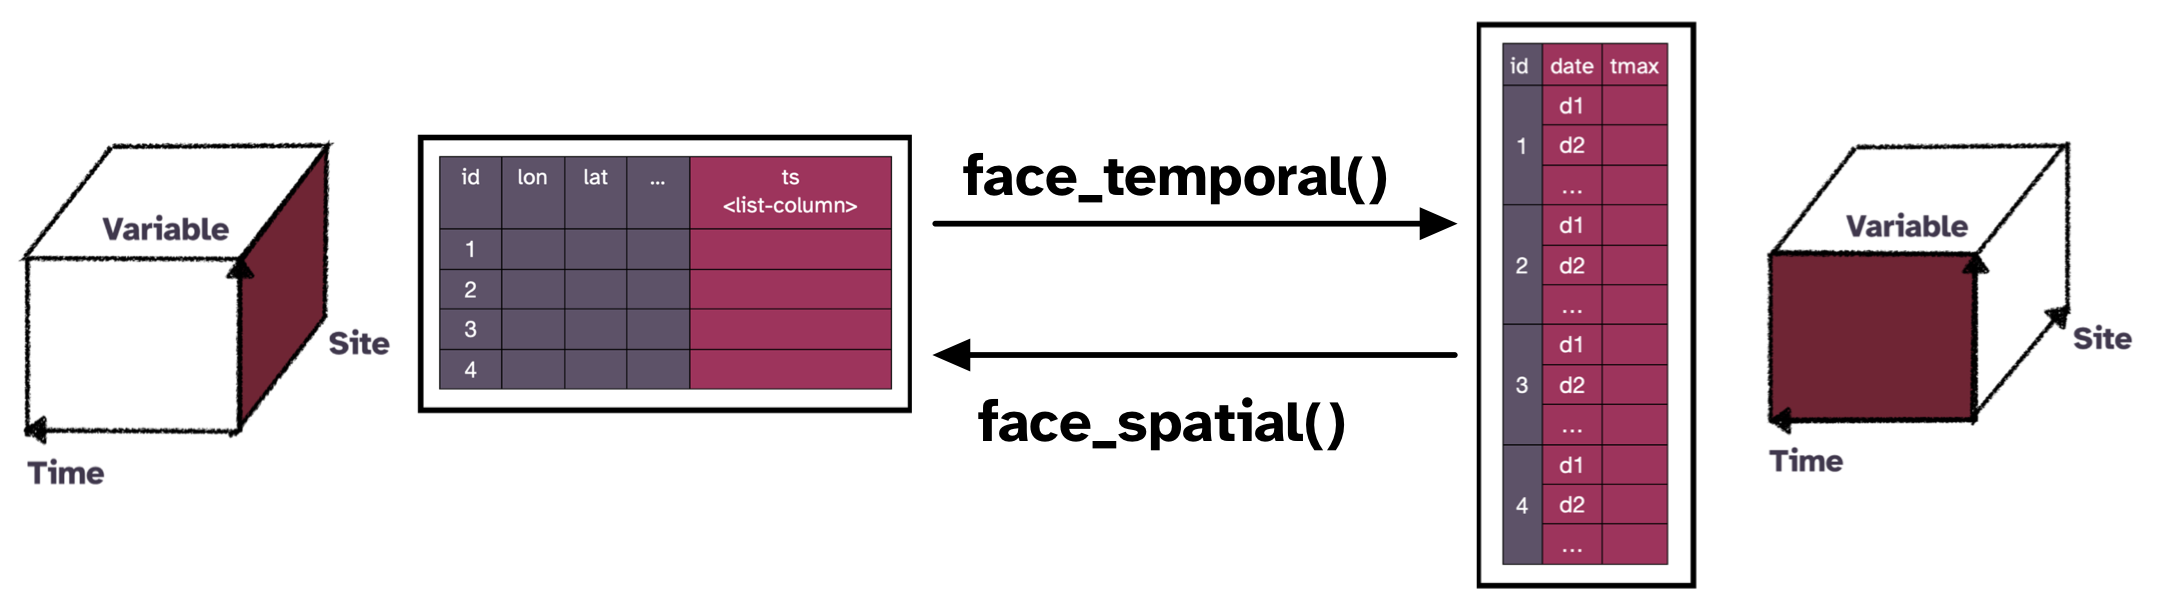
\includegraphics[width=1\linewidth]{/Users/pmen0008/Desktop/paper-cubble/figures/diagram-keynotes/diagram-keynotes.001} 

}

\caption{An illustration of the functions \code{face\_temporal()} and \code{face\_spatial()}: \code{face\_temporal()} converts a spatial cubble into a temporal cubble to focus on the temporal variables. Conversely, \code{face\_spatial()} transforms a temporal cubble into a spatial one to focus on the spatial variables.}\label{fig:face}
\end{figure}
\end{CodeChunk}

\hypertarget{compatibility-with-tsibble-and-sf}{%
\subsection{Compatibility with tsibble and sf}\label{compatibility-with-tsibble-and-sf}}

Analysts often have their preferred spatial or temporal data structure for spatial or temporal analysis, which they may wish to continue using for spatio-temporal analysis. With \code{cubble}, analysts can incorporate the \code{tsibble} class \citep{tsibble} in a temporal cubble and the \code{sf} class \citep{sf} in a spatial cubble.

\hypertarget{using-a-tsibble-object-as-the-temporal-component}{%
\subsubsection{Using a tsibble object as the temporal component}\label{using-a-tsibble-object-as-the-temporal-component}}

The \code{key} and \code{index} arguments in a \code{cubble} object corresponds to the \code{tsibble} counterparts and they can be safely omitted, if the temporal component is a \code{tsibble} object, i.e.~\code{meteo_ts} in the example below. The \code{tsibble} class (\code{tbl_ts}) from the input will be carried over to the temporal cubble, indicated by the \code{[tsibble]} in the header and in the object class:

\begin{CodeChunk}
\begin{CodeInput}
R> ts_nested <- make_cubble(
+   spatial = stations, temporal = meteo_ts, coords = c(long, lat))
R> (ts_long <- face_temporal(ts_nested))
\end{CodeInput}
\begin{CodeOutput}
# cubble:   key: id [3], index: date, long form, [tsibble]
# temporal: 2020-01-01 -- 2020-01-10 [1D], no gaps
# spatial:  long [dbl], lat [dbl], elev [dbl], name [chr], wmo_id [dbl]
  id          date        prcp  tmax  tmin
  <chr>       <date>     <dbl> <dbl> <dbl>
1 ASN00086038 2020-01-01     0  26.8  11  
2 ASN00086038 2020-01-02     0  26.3  12.2
3 ASN00086038 2020-01-03     0  34.5  12.7
4 ASN00086038 2020-01-04     0  29.3  18.8
5 ASN00086038 2020-01-05    18  16.1  12.5
# i 25 more rows
\end{CodeOutput}
\begin{CodeInput}
R> class(ts_long)
\end{CodeInput}
\begin{CodeOutput}
[1] "temporal_cubble_df" "cubble_df"          "tbl_ts"            
[4] "tbl_df"             "tbl"                "data.frame"        
\end{CodeOutput}
\end{CodeChunk}

Methods applied to the \code{tbl_ts} class can also be applied to the temporal cubble objects, for example, checking whether the data contain temporal gaps:

\begin{CodeChunk}
\begin{CodeInput}
R> ts_long |> has_gaps()
\end{CodeInput}
\begin{CodeOutput}
# A tibble: 3 x 2
  id          .gaps
  <chr>       <lgl>
1 ASN00086038 FALSE
2 ASN00086077 FALSE
3 ASN00086282 FALSE
\end{CodeOutput}
\end{CodeChunk}

A created temporal cubble can promote its temporal component to a \code{tsibble} object using \code{make_temporal_tsibble()}. See the code example below using the \code{cb_long} object created in Section \ref{create}:

\begin{CodeChunk}
\begin{CodeInput}
R> cb_long |> make_temporal_tsibble() 
\end{CodeInput}
\begin{CodeOutput}
# cubble:   key: id [3], index: date, long form, [tsibble]
# temporal: 2020-01-01 -- 2020-01-10 [1D], no gaps
# spatial:  long [dbl], lat [dbl], elev [dbl], name [chr], wmo_id [dbl]
  id          date        prcp  tmax  tmin
  <chr>       <date>     <dbl> <dbl> <dbl>
1 ASN00086038 2020-01-01     0  26.8  11  
2 ASN00086038 2020-01-02     0  26.3  12.2
3 ASN00086038 2020-01-03     0  34.5  12.7
4 ASN00086038 2020-01-04     0  29.3  18.8
5 ASN00086038 2020-01-05    18  16.1  12.5
# i 25 more rows
\end{CodeOutput}
\end{CodeChunk}

\hypertarget{using-an-sf-object-as-the-spatial-component}{%
\subsubsection{Using an sf object as the spatial component}\label{using-an-sf-object-as-the-spatial-component}}

Similarly, the spatial component of a cubble object can be an \code{sf} object and if the \code{coords} argument is omitted, it will be calculated from the sf geometry. The sf status is signalled by the \code{[sf]} label in the cubble header:

\begin{CodeChunk}
\begin{CodeInput}
R> (sf_nested <- make_cubble(
+   spatial = stations_sf, temporal = meteo, 
+   key = id, index = date))
\end{CodeInput}
\begin{CodeOutput}
# cubble:   key: id [3], index: date, nested form, [sf]
# spatial:  [144.8321, -37.98, 145.0964, -37.6655], WGS 84
# temporal: date [date], prcp [dbl], tmax [dbl], tmin [dbl]
  id           elev name   wmo_id  long   lat            geometry ts      
  <chr>       <dbl> <chr>   <dbl> <dbl> <dbl>         <POINT [°]> <list>  
1 ASN00086038  78.4 essen~  95866  145. -37.7 (144.9066 -37.7276) <tibble>
2 ASN00086077  12.1 moora~  94870  145. -38.0   (145.0964 -37.98) <tibble>
3 ASN00086282 113.  melbo~  94866  145. -37.7 (144.8321 -37.6655) <tibble>
\end{CodeOutput}
\begin{CodeInput}
R> class(sf_nested)
\end{CodeInput}
\begin{CodeOutput}
[1] "spatial_cubble_df" "cubble_df"         "sf"               
[4] "tbl_df"            "tbl"               "data.frame"       
\end{CodeOutput}
\end{CodeChunk}

This allows applying functions from the \code{sf} package to a cubble object, for example, to handle coordinate transformation with \code{st_transform}:

\begin{CodeChunk}
\begin{CodeInput}
R> sf_nested |> sf::st_transform(crs = "EPSG:3857")
\end{CodeInput}
\begin{CodeOutput}
# cubble:   key: id [3], index: date, nested form, [sf]
# spatial:  [16122635.6225205, -4576600.8687746, 16152057.3639371,
#   -4532279.35567565], WGS 84
# temporal: date [date], prcp [dbl], tmax [dbl], tmin [dbl]
  id           elev name   wmo_id  long   lat            geometry ts      
  <chr>       <dbl> <chr>   <dbl> <dbl> <dbl>         <POINT [°]> <list>  
1 ASN00086038  78.4 essen~  95866  145. -37.7 (16130929 -4541016) <tibble>
2 ASN00086077  12.1 moora~  94870  145. -38.0 (16152057 -4576601) <tibble>
3 ASN00086282 113.  melbo~  94866  145. -37.7 (16122636 -4532279) <tibble>
\end{CodeOutput}
\end{CodeChunk}

The spatial component of a created \code{cubble} can also be promoted into an \code{sf} object with \code{make_spatial_sf()}:

\begin{CodeChunk}
\begin{CodeInput}
R> cb_nested |> make_spatial_sf() 
\end{CodeInput}
\begin{CodeOutput}
# cubble:   key: id [3], index: date, nested form, [sf]
# spatial:  [144.8321, -37.98, 145.0964, -37.6655], WGS 84
# temporal: date [date], prcp [dbl], tmax [dbl], tmin [dbl]
  id           long   lat  elev name   wmo_id ts                  geometry
  <chr>       <dbl> <dbl> <dbl> <chr>   <dbl> <list>           <POINT [°]>
1 ASN00086038  145. -37.7  78.4 essen~  95866 <tibble> (144.9066 -37.7276)
2 ASN00086077  145. -38.0  12.1 moora~  94870 <tibble>   (145.0964 -37.98)
3 ASN00086282  145. -37.7 113.  melbo~  94866 <tibble> (144.8321 -37.6655)
\end{CodeOutput}
\end{CodeChunk}

\hypertarget{tidyverse}{%
\subsection{Comparison to other spatio-temporal classes}\label{tidyverse}}

In \proglang{R}, there are other existing spatio-temporal data structure and this section compares and contrasts \pkg{cubble} with other existing alternatives, specifically \pkg{stars} and \pkg{sftime}. The \pkg{stars} package \citep{stars} uses an array structure, as oppose to tibble, to represent multivariate spatio-temporal data. While both \pkg{stars} and \pkg{cubble} support vector and raster data, it is a matter of choice on which structure to use given the application. Analysts working on satellite imageries may prefer the array structure in \pkg{stars}, while others originally working with spatio-temporal data in 2D data frames may find \pkg{cubble} easier to adopt from their existing computing workflow.

The \pkg{sftime} package \citep{sftime} also builds from a tibble object and its focus is on handling irregular spatio-temporal data. This means \pkg{sftime} can also handle full space-time grids and sparse space-time layouts represented in \pkg{cubble}. However, \pkg{cubble} uses nesting to avoid storing spatial variables repetitively at each timestamp. This provides memory efficiency when data is observed frequent, i.e.~daily or sub-daily, or the spatial geometry is computationally expensive to store repeatedly, i.e.~polygons or multipolygons. Consider the \code{climate_aus} data in the \pkg{cubble} package with 639 stations observed daily throughout the year 2020. In that case, the \code{sftime} object is approximately 14 times larger than the corresponding \code{cubble} object (118 MB vs.~8.5 MB).

\hypertarget{others}{%
\section{Other features and considerations}\label{others}}

\hypertarget{matching}{%
\subsection{Data fusion and matching}\label{matching}}

Matching time series from an old list of stations to a new list is a common task in spatio-temporal data analysis. In cubble, matching based on distance and time series features can be performed using the functions \texttt{match\_spatial()} and \texttt{match\_temporal()}. The \texttt{match\_spatial()} function finds the matched pairs in two cubble objects based on distance between sites:

\begin{verbatim}
match_spatial(<cubble_obj1>, <cubble_obj2>, ...)
\end{verbatim}

Two arguments are available to control the outputs: the argument \texttt{spatial\_n\_group} specifies the number of paired groups to output and the argument \texttt{spatial\_n\_each} specifies the number of each for each item in the first cubble object (default to 1 for one-to-one matching).

The function \texttt{match\_temporal()} takes the outputs from spatial matching and calculates a similarity score of the time series between spatially matched pairs. The temporal matching requires two identifiers: one for separating each spatially matched group: \texttt{match\_id} and one for separating the two data sources: \texttt{data\_id}. Matching between different variables can be specified using the \texttt{temporal\_by} argument, similar to the \texttt{by} syntax from dplyr's \texttt{*\_join}.

\begin{verbatim}
match_temporal(
  <obj_from_match_spatial>, 
  data_id = ... , match_id = ..., 
  temporal_by = c("..." = "...")
)
\end{verbatim}

The similarity score between two time series is calculated using a matching function, which can be customised by the analysts based on the time series feature relevant to match. The matching function takes two time series as a list and returns a single numerical score. By default, cubble uses a simple peak matching algorithm (\texttt{match\_peak}) to count the number of peaks in two time series that fall within a specified temporal window.

\hypertarget{interactive-graphics}{%
\subsection{Interactive graphics}\label{interactive-graphics}}

The cubble workflow can be easily incorporated into an interactive graphics pipeline (e.g., \citet{buja1988elements}; \citet{buja1996interactive}; \citet{sutherland2000orca}; \citet{xie2014reactive}; \citet{cheng2016enabling}). This section describes the linking between a map and multiple time series in a \code{cubble} object using the package \pkg{crosstalk} \citep{crosstalk}, as illustrated in Figure \ref{fig:illu-interactive}. The spatial and temporal cubble can be constructed as a shared crosstalk object to create a link between a map and a time series plot. For instance, when a user selects a location on the map as shown on panel (a), the corresponding site is highlighted. This selection activates a row in the spatial cubble, which is then connected to the temporal cubble, resulting in the selection of all observations with the same ID as depicted in panel (b). Consequently the temporal cubble highlights the corresponding series in the time series plot displayed in panel (c). The linking can also be initiated from the time series plot by selecting points on the time series graph. This action selects rows with the same ID in the temporal cubble and the corresponding row in the spatial cubble so that points can be highlight on the map.

\begin{CodeChunk}
\begin{figure}

{\centering 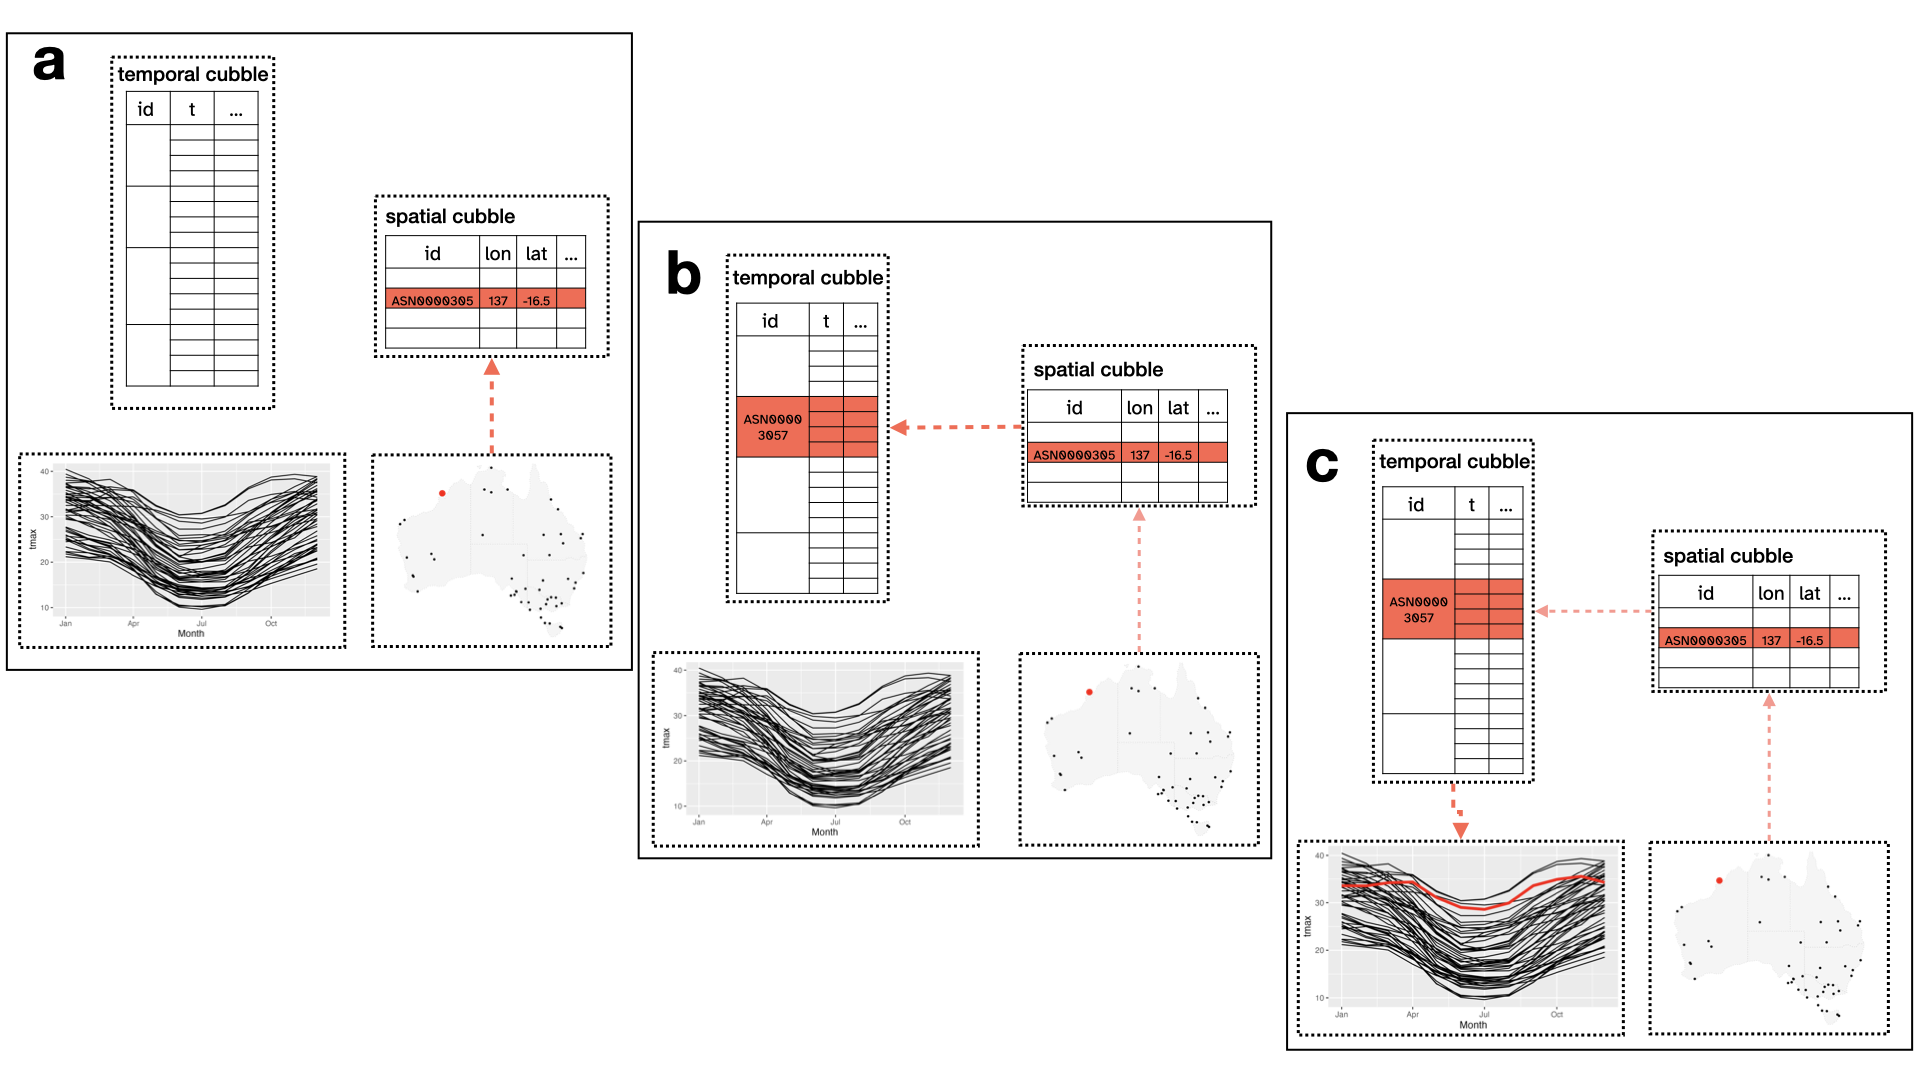
\includegraphics[width=1\linewidth,height=0.35\textheight]{/Users/pmen0008/Desktop/paper-cubble/figures/diagram-keynotes/‎diagram-keynotes.‎002} 

}

\caption{Linking between multiple plots. The line plots and the map are constructed from shared \code{crosstalk} objects. When a station is selected on the map (a), the corresponding row in the spatial \code{cubble} will be activated. This will link to all the rows with the same id in the temporal \code{cubble} (b) and update the line plot (c).}\label{fig:illu-interactive}
\end{figure}
\end{CodeChunk}

\hypertarget{st_transformation}{%
\subsection{Spatio-temporal transformations}\label{st_transformation}}

Visualizing spatio-temporal data is important for exploring and understanding the data at hand, aiding in decision-making, and facilitating effective communication. To collectively visualize spatial and temporal information, several options are available such as: faceted maps across time, map animations, or interactive graphics that link maps and time series plots among others. Faceted maps and spatio-temporal animations, while commonly used, may be difficult to compare across time and space since users need to inspect multiple facets or frames to find changes in time or space. The glyph map \citep{Wickham2012-yr} resolves this issue by imposing the time series onto the map as a glyph through a coordinate transformation. The transformation uses linear algebra to convert the temporal coordinates (minor coordinates) into the spatial coordinates (major coordinates) and is implemented in the package \texttt{GGally} \citep{ggally}. The \pkg{cubble} package provides a ggproto implementation to create glyph maps, \texttt{geom\_glyph()} and it takes four required aestheticsf : \texttt{x\_major}, \texttt{y\_major}, \texttt{x\_minor}, and \texttt{y\_minor}:

\begin{verbatim}
data |> 
  ggplot() +
  geom_glyph(aes(x_major = ..., x_minor = ..., 
                 y_major = ..., y_minor = ...))
\end{verbatim}

Other useful controls to modify the glyph map that can be include are:

\begin{itemize}
\tightlist
\item
  the implementation of a polar coordinate glyph maps with \code{polar = TRUE},
\item
  the adjustment of the glyph size arguments using \code{width} and \code{height},
\item
  a transformation relative to the all series (\code{global_rescale} defaults to \code{TRUE}) or each single series, and
\item
  the XX of the reference boxes and lines with \code{geom_glyph_box()} and \code{geom_glyph_line()}.
\end{itemize}

\hypertarget{examples}{%
\section{Applications}\label{examples}}

Five examples are chosen to illustrate different aspects of the \pkg{cubble} package: creating a \code{cubble} object from two Coronavirus (COVID) data tables with the challenge of having different location names, using spatial transformations to make a glyph map of seasonal temperature changes, matching river level data with weather station records to analyze water supply, reading NetCDF format data to replicate a climate reanalysis plot, and demonstrating the workflow to create complex interactive linked plots.

\hypertarget{covid}{%
\subsection{Victoria COVID spatio-temporal incidence and spread}\label{covid}}

Since the start of the COVID-19 pandemic, the Victoria State Government in Australia has been providing daily COVID-19 case counts per Local Government Area (LGA). This data can be combined with map polygon data, available from the Australian Bureau of Statistics (ABS), to visualize COVID-19 incidence and spread. In the \pkg{cubble} package, the COVID-19 count data (\code{covid}) and the LGA information (\code{lga}) are available as a \code{tsibble} object and an \code{sf} object respectively. A cubble object can be created from these two component using \code{make_cubble()}. The \code{id} column containing LGA information has different names in the two data sets and that can be specified via the \code{by} argument:

\begin{CodeChunk}
\begin{CodeInput}
R> cb <- make_cubble(lga, covid, by = c("lga_name_2018" = "lga"))
\end{CodeInput}
\begin{CodeOutput}
Warning: st_centroid assumes attributes are constant over geometries
\end{CodeOutput}
\begin{CodeOutput}
! Some sites in the spatial table don't have temporal information
\end{CodeOutput}
\begin{CodeOutput}
! Some sites in the temporal table don't have spatial information
\end{CodeOutput}
\begin{CodeOutput}
! Use `check_key()` to check on the unmatched key
The cubble is created only with sites having both spatial and
temporal information
\end{CodeOutput}
\end{CodeChunk}

The difference in LGA naming between both data sets triggers cubble to issue a warning, alerting the user to this discrepancy. The warning message suggests there are some differences between the LGA encoding used by Victoria government and ABS and prompts analysts to check the mismatch using \code{check_key()}:

\begin{CodeChunk}
\begin{CodeInput}
R> (check_res <- check_key(
+   spatial = lga, temporal = covid, 
+   by = c("lga_name_2018" = "lga")
+ ))
\end{CodeInput}
\begin{CodeOutput}
$paired
# A tibble: 78 x 2
  spatial        temporal      
  <chr>          <chr>         
1 Alpine (S)     Alpine (S)    
2 Ararat (RC)    Ararat (RC)   
3 Ballarat (C)   Ballarat (C)  
4 Banyule (C)    Banyule (C)   
5 Bass Coast (S) Bass Coast (S)
# i 73 more rows

$potential_pairs
# A tibble: 2 x 2
  spatial             temporal    
  <chr>               <chr>       
1 Kingston (C) (Vic.) Kingston (C)
2 Latrobe (C) (Vic.)  Latrobe (C) 

$others
$others$spatial
character(0)

$others$temporal
[1] "Interstate" "Overseas"   "Unknown"   
\end{CodeOutput}
\end{CodeChunk}

The result of the \code{check_key()} function is a list containing three elements: 1) matched keys from both tables, 2) potentially paired keys, and 3) others (XXX what is others exactly?). Here, the main mismatch arises from the two LGAs: Kingston and Latrobe (Kingston is a LGA in both Victoria and South Australia and Latrobe is a LGA in both Victoria and Tasmania). Analysts can then reconcile the spatial and temporal data based on this check summary and recreate the cubble object:

\begin{CodeChunk}
\begin{CodeInput}
R> lga2 <- lga |>
+   rename(lga = lga_name_2018) |> 
+   mutate(lga = ifelse(lga == "Kingston (C) (Vic.)", "Kingston (C)", lga),
+          lga = ifelse(lga == "Latrobe (C) (Vic.)", "Latrobe (C)", lga))
R>   
R> covid2 <- covid |> filter(!lga %in% check_res$others$temporal)
R> 
R> (cb <- make_cubble(spatial = lga2, temporal = covid2))
\end{CodeInput}
\begin{CodeOutput}
# cubble:   key: lga [80], index: date, nested form, [sf]
# spatial:  [140.961682, -39.1339581, 149.976291, -33.9960517], WGS 84
# temporal: date [date], n [dbl], avg_7day [dbl]
  lga             long   lat                                   geometry ts      
  <chr>          <dbl> <dbl>                             <GEOMETRY [°]> <list>  
1 Alpine (S)      147. -36.9 POLYGON ((146.7258 -36.45922, 146.7198 -3~ <tbl_ts>
2 Ararat (RC)     143. -37.5 POLYGON ((143.1807 -37.73152, 143.0609 -3~ <tbl_ts>
3 Ballarat (C)    144. -37.5 POLYGON ((143.6622 -37.57241, 143.68 -37.~ <tbl_ts>
4 Banyule (C)     145. -37.7 POLYGON ((145.1357 -37.74091, 145.1437 -3~ <tbl_ts>
5 Bass Coast (S)  146. -38.5 MULTIPOLYGON (((145.5207 -38.30667, 145.5~ <tbl_ts>
# i 75 more rows
\end{CodeOutput}
\end{CodeChunk}

\hypertarget{historicaltmax}{%
\subsection{Australian historical maximum temperature}\label{historicaltmax}}

The Global Historical Climatology Network (GHCN) provides daily climate measures for stations worldwide. In the \pkg{cubble} package, the cubble object \code{historical_tmax} contains daily maximum temperature data for 75 stations in Australia, covering two periods: 1971-1975 and 2016-2020. This example uses glyph maps to compare the changes in temperature between these two periods.

To prevent overlapping of weather stations on the map, stations are selected to ensure a minimum distance of 50km. Distance between stations can be calculated with \code{sf::st_distance()} after turning the spatial cubble to also be an sf object with \code{make_spatial_sf()}:

\begin{CodeChunk}
\begin{CodeInput}
R> a <- historical_tmax |> make_spatial_sf() |> st_distance()
R> a[upper.tri(a, diag = TRUE)] <- 1e6
R> 
R> (tmax <- historical_tmax |> 
+   filter(rowSums(a < units::as_units(50, "km")) == 0))
\end{CodeInput}
\begin{CodeOutput}
# cubble:   key: id [54], index: date, nested form
# spatial:  [141.2652, -39.1297, 153.3633, -28.9786], Missing CRS!
# temporal: date [date], tmax [dbl]
  id           long   lat  elev name                     wmo_id ts      
  <chr>       <dbl> <dbl> <dbl> <chr>                     <dbl> <list>  
1 ASN00047016  141. -34.0    43 lake victoria storage     94692 <tibble>
2 ASN00047019  142. -32.4    61 menindee post office      94694 <tibble>
3 ASN00048015  147. -30.0   115 brewarrina hospital       95512 <tibble>
4 ASN00048027  146. -31.5   260 cobar mo                  94711 <tibble>
5 ASN00048031  149. -29.5   145 collarenebri (albert st)  95520 <tibble>
# i 49 more rows
\end{CodeOutput}
\end{CodeChunk}

Daily maximum temperature is then averaged into monthly series for each periods in the temporal cubble. The last step with \code{unfold()} moves the two coordinate columns (\code{long, lat}) into the temporal cubble, preparing the data for the glyph map:

\begin{CodeChunk}
\begin{CodeInput}
R> (tmax <- tmax |>
+   face_temporal() |> 
+   group_by(
+     yearmonth = tsibble::make_yearmonth(
+       year = ifelse(lubridate::year(date) > 2015, 2016, 1971),
+       month = lubridate::month(date))
+   )|>
+   summarise(tmax = mean(tmax, na.rm = TRUE)) |> 
+   mutate(group = as.factor(lubridate::year(yearmonth)),
+          month = lubridate::month(yearmonth)) |> 
+   unfold(long, lat))
\end{CodeInput}
\begin{CodeOutput}
# cubble:   key: id [54], index: yearmonth, long form
# temporal: 1971 Jan -- 2016 Dec [1M], has gaps!
# spatial:  long [dbl], lat [dbl], elev [dbl], name [chr], wmo_id [dbl]
  yearmonth id           tmax group month  long   lat
      <mth> <chr>       <dbl> <fct> <dbl> <dbl> <dbl>
1  1971 Jan ASN00047016  31.1 1971      1  141. -34.0
2  1971 Jan ASN00047019  33.1 1971      1  142. -32.4
3  1971 Jan ASN00048015  33.9 1971      1  147. -30.0
4  1971 Jan ASN00048027  32.5 1971      1  146. -31.5
5  1971 Jan ASN00048031  33.3 1971      1  149. -29.5
# i 1,276 more rows
\end{CodeOutput}
\end{CodeChunk}

A quick check on the number of observations for each location is made, revealing that there are several with less than 24 observations -- these stations lack temperature values for some months. In this example, those stations are removed by switching to the spatial \code{cubble} to operate on the spatial component over time, and then, move back into the temporal \code{cubble} (to make the glyph map):

\begin{CodeChunk}
\begin{CodeInput}
R> tmax <- tmax |> 
+   face_spatial() |> 
+   rowwise() |>
+   filter(nrow(ts) == 24) |>
+   face_temporal()
\end{CodeInput}
\end{CodeChunk}

The following code creates the glyph map (a) in Figure \ref{fig:glyphmap} (additional codes are needed for highlighting the single station, Cobar and styling) and the glyph map (c) is produced similarly with the difference series, rather than the two original series, being plotted.

\begin{verbatim}
nsw_vic <- ozmaps::abs_ste |> 
  filter(NAME %in% c("Victoria","New South Wales"))

tmax |> 
  ggplot(aes(x_major = long, x_minor = month, 
             y_major = lat, y_minor = tmax,
             group = interaction(id, group))) + 
  geom_sf(data =  nsw_vic, ...,  inherit.aes = FALSE) + 
  geom_glyph_box(width = 0.8, height = 0.3) + 
  geom_glyph(aes(color = group), width = 0.8, height = 0.3) +
  ...
\end{verbatim}

\begin{CodeChunk}
\begin{figure}

{\centering 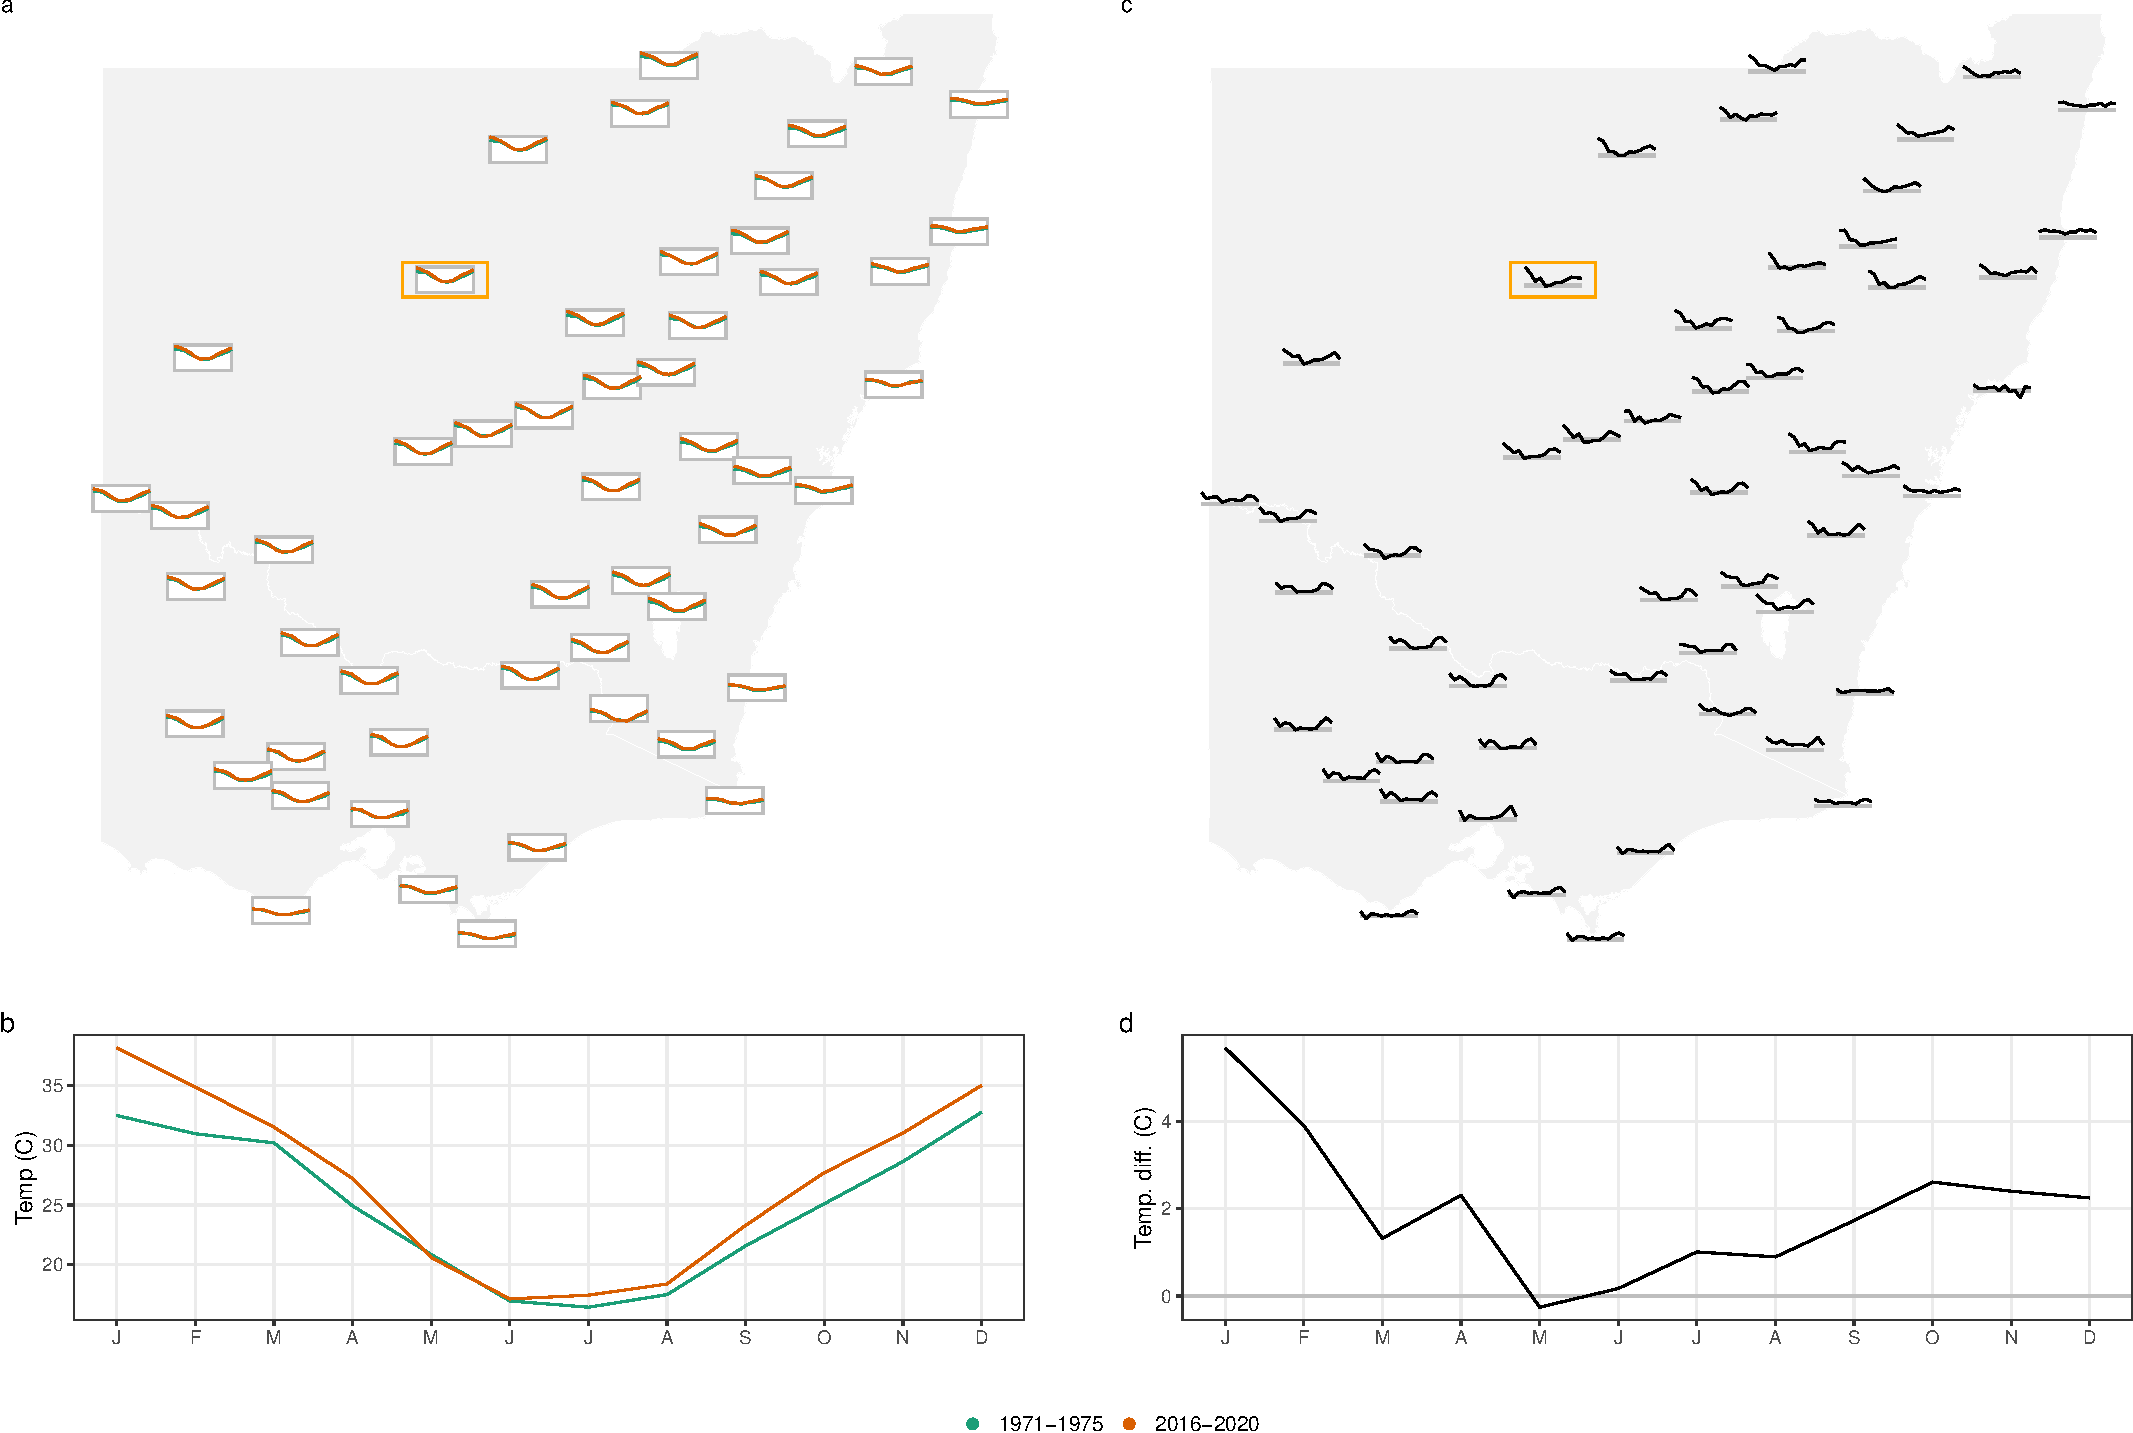
\includegraphics[width=1\linewidth]{/Users/pmen0008/Desktop/paper-cubble/figures/glyphmap-1} 

}

\caption[Comparison of average maximum temperature between 1971-1975 and 2016-2020 for 54 stations in Victoria and New South Wales, Australia]{Comparison of average maximum temperature between 1971-1975 and 2016-2020 for 54 stations in Victoria and New South Wales, Australia. (a) and (b): the monthly temperature series for the two periods in a glyph map and for a single station Cobar, highlighted in orange in the glyph map. (c) and (d): the difference series between the two periods (2016s minus 1971s) in a glyph map and for station Cobar. The grey horizontal line marks zero difference. The glyph map displaying the difference series (c) reveals more pronounced changes between the two periods, with many inland locations in New South Wales show an increased temperature in late summer (Jan-Feb) in recent years.}\label{fig:glyphmap}
\end{figure}
\end{CodeChunk}

\hypertarget{river-levels-and-rainfall-in-victoria}{%
\subsection{River levels and rainfall in Victoria}\label{river-levels-and-rainfall-in-victoria}}

The Bureau of Meteorology collects water level data and they can be matched with the precipitation data from the climate weather stations. The data \texttt{river} from the \pkg{cubble} package contains water course level data for 71 river gauges collected in Victoria, Australia. Victoria weather station data can be subsetted from the \texttt{climate\_aus} data in \pkg{cubble}.

\begin{CodeChunk}
\begin{CodeInput}
R> climate_vic <- climate_aus |>
+   filter(between(as.numeric(substr(id, 7, 8)), 76, 90)) |>
+   mutate(type = "climate")
R> river <- cubble::river |> mutate(type = "river") 
\end{CodeInput}
\end{CodeChunk}

Spatial match on the site location is first performed since rainfall can directly impact water level in the nearby river. With \code{match_spatial()}, we can obtain a summary of the 10 closest pairs:

\begin{CodeChunk}
\begin{CodeInput}
R> res_sp <- match_spatial(climate_vic, river, spatial_n_group = 10)
R> print(res_sp, n = 20)
\end{CodeInput}
\begin{CodeOutput}
# A tibble: 10 x 4
   from        to      dist group
   <chr>       <chr>    [m] <int>
 1 ASN00088051 406213 1838.     1
 2 ASN00084145 222201 2185.     2
 3 ASN00085072 226027 3282.     3
 4 ASN00080015 406704 4034.     4
 5 ASN00085298 226027 4207.     5
 6 ASN00082042 405234 6153.     6
 7 ASN00086038 230200 6167.     7
 8 ASN00086282 230200 6928.     8
 9 ASN00085279 224217 7431.     9
10 ASN00080091 406756 7460.    10
\end{CodeOutput}
\end{CodeChunk}

The result can also be returned as a list of matched cubbles, by setting the argument \code{return_cubble = TRUE}. All the results can be combined into a single cubble using \code{bind_rows()}, after excluding the two pairs where a river station is matched to more than one weather stations (river station \texttt{226027} is matched twice in group 3 and 5 and similarly for station \texttt{230200} in group 7 and 8).

\begin{CodeChunk}
\begin{CodeInput}
R> res_sp <- match_spatial(
+   climate_vic, river, 
+   spatial_n_group = 10, return_cubble = TRUE)
R> (res_sp <- res_sp[-c(5, 8)] |> bind_rows())
\end{CodeInput}
\begin{CodeOutput}
# cubble:   key: id [16], index: date, nested form, [sf]
# spatial:  [144.5203, -38.144913, 148.4667, -36.128657], WGS 84
# temporal: date [date], prcp [dbl], tmax [dbl], tmin [dbl]
  id      long   lat  elev name  wmo_id ts       type              geometry
  <chr>  <dbl> <dbl> <dbl> <chr>  <dbl> <list>   <chr>          <POINT [°]>
1 ASN00~  145. -37.0 290   rede~  94859 <tibble> clim~  (144.5203 -37.0194)
2 406213  145. -37.0  NA   CAMP~     NA <tibble> river (144.5403 -37.01512)
3 ASN00~  148. -37.7  62.7 orbo~  95918 <tibble> clim~  (148.4667 -37.6922)
4 222201  148. -37.7  NA   SNOW~     NA <tibble> river  (148.451 -37.70739)
5 ASN00~  147. -38.1   4.6 east~  94907 <tibble> clim~  (147.1322 -38.1156)
# i 11 more rows
# i 2 more variables: group <int>, dist [m]
\end{CodeOutput}
\end{CodeChunk}

To match the water level series with precipitation, the function \code{match_temporal()} is used with the variable \code{group} and \code{types} identifying the matching group and the two data sources:

\begin{CodeChunk}
\begin{CodeInput}
R> (res_tm <- res_sp |> 
+   match_temporal(
+     data_id = type, match_id = group,
+     temporal_by = c("prcp" = "Water_course_level")))
\end{CodeInput}
\begin{CodeOutput}
# A tibble: 8 x 2
  group match_res
  <int>     <dbl>
1     1        30
2     2         5
3     3        14
4     4        20
5     6        23
# i 3 more rows
\end{CodeOutput}
\end{CodeChunk}

Similarly, the cubble output can be returned using the argument \texttt{return\_cubble\ =\ TRUE}. Here we select the four pairs with the highest number of matching peaks and show them on the map (a) and as standardized series (b) in Figure \ref{fig:matching}.

\begin{CodeChunk}
\begin{CodeInput}
R> res_tm <- res_sp |> 
+   match_temporal(
+     data_id = type, match_id = group,
+     temporal_by = c("prcp" = "Water_course_level"),
+     return_cubble = TRUE)
R> (res_tm <- res_tm |> bind_rows() |> filter(group %in% c(1, 7, 6, 9)))
\end{CodeInput}
\begin{CodeOutput}
# cubble:   key: id [8], index: date, nested form, [sf]
# spatial:  [144.5203, -37.8817, 147.572223, -36.8472], WGS 84
# temporal: date [date], matched [dbl]
  id         long   lat  elev name  wmo_id type              geometry group
  <chr>     <dbl> <dbl> <dbl> <chr>  <dbl> <chr>          <POINT [°]> <int>
1 ASN00088~  145. -37.0 290   rede~  94859 clim~  (144.5203 -37.0194)     1
2 406213     145. -37.0  NA   CAMP~     NA river (144.5403 -37.01512)     1
3 ASN00082~  146. -36.8 502   stra~  95843 clim~  (145.7308 -36.8472)     6
4 405234     146. -36.9  NA   SEVE~     NA river (145.6828 -36.88701)     6
5 ASN00086~  145. -37.7  78.4 esse~  95866 clim~  (144.9066 -37.7276)     7
# i 3 more rows
# i 3 more variables: dist [m], ts <list>, match_res <dbl>
\end{CodeOutput}
\end{CodeChunk}

\begin{CodeChunk}
\begin{figure}

{\centering 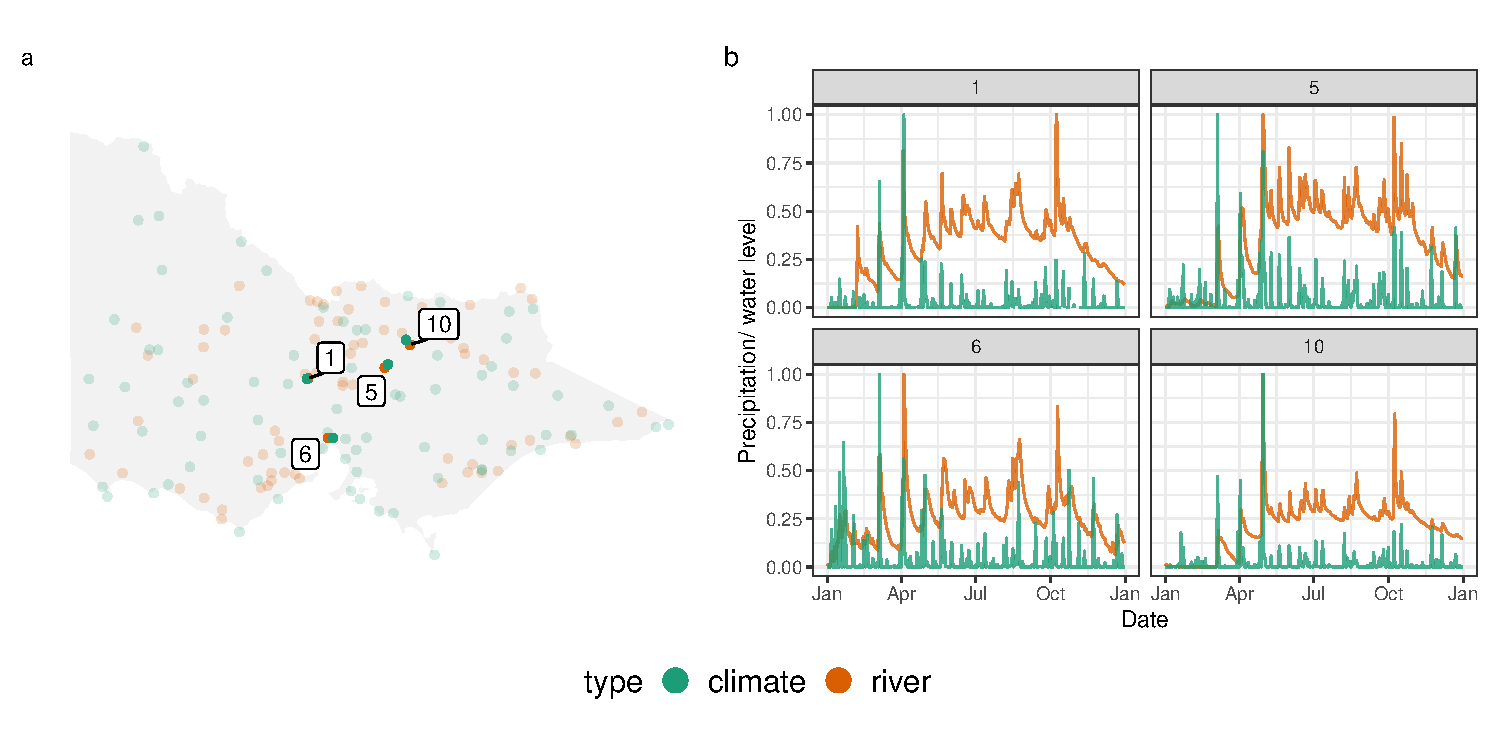
\includegraphics[width=1\linewidth]{/Users/pmen0008/Desktop/paper-cubble/figures/matching-1} 

}

\caption[Matched weather stations and river gauges on the map (a) and across time (b)]{Matched weather stations and river gauges on the map (a) and across time (b). Precipitation and water level have been standardised between 0 and 1 to be displayed in the same scale in (b). The water level reflects the increase in precipitation.}\label{fig:matching}
\end{figure}
\end{CodeChunk}

\hypertarget{era5-climate-reanalysis-data}{%
\subsection{ERA5: climate reanalysis data}\label{era5-climate-reanalysis-data}}

The ERA5 reanalysis \citep{hersbach2020era5} provides hourly estimates of atmospheric, land and oceanic climate variables on a global scale and is available in the NetCDF format from Copernicus Climate Data Store (CDS). This example reproduces Figure 19 in the \citet{hersbach2020era5} paper with cubble, in Figure \ref{fig:netcdf}. The plot shows the southern polar vortex splitting into two on 2002-09-26, and further splitting into four on 2002-10-04. Further explanation of why this is interesting can be found in the figure source, and also in \citet{simmons2020global} and \citet{simmons2005ecmwf}.

A \code{ncdf4} object \citep{ncdf4} can be converted into a cubble using \code{as_cubble()} and the NetCDF data can be subsetted with arguments \code{vars}, \code{long_range} and \code{lat_range}. In this example, the variables q (specific humidity) and z (geopotential) are read in and the coordinates are subsetted to every degree in longitude and latitude:

\begin{CodeChunk}
\begin{CodeInput}
R> raw <- ncdf4::nc_open(here::here("data/era5-pressure.nc"))
R> (dt <- as_cubble(
+   raw, vars = c("q", "z"),
+   long_range = seq(-180, 180, 1), lat_range = seq(-88, -15, 1)))
\end{CodeInput}
\begin{CodeOutput}
# cubble:   key: id [26640], index: time, nested form
# spatial:  [-180, -88, 179, -15], Missing CRS!
# temporal: time [date], q [dbl], z [dbl]
     id  long   lat ts              
  <int> <dbl> <dbl> <list>          
1     1  -180   -15 <tibble [8 x 3]>
2     2  -179   -15 <tibble [8 x 3]>
3     3  -178   -15 <tibble [8 x 3]>
4     4  -177   -15 <tibble [8 x 3]>
5     5  -176   -15 <tibble [8 x 3]>
# i 26,635 more rows
\end{CodeOutput}
\end{CodeChunk}

Once the NetCDF data is coerced into a cubble object, subsequent analysis can be conducted to filter on the date of interest, scale the variable specific humidity and create visualisation in ggplot to reproduce the ERA5 plot. A snippet of code to create Figure \ref{fig:netcdf} is provided below with additional codes needed to style the plot

\begin{verbatim}
res <- dt |> 
  face_temporal() |> 
  filter(lubridate::date(time) %in% 
           as.Date(c("2002-09-22", "2002-09-26",
                     "2002-09-30", "2002-10-04"))) |>
  unfold(long, lat) |> 
  mutate(q = q* 10^6)

con <- rnaturalearth::ne_coastline("small", returnclass = "sf")
box <- st_bbox(c(xmin = -180, ymin = -90, xmax = 180, ymax = -15), crs = st_crs(con)) 
country <- con |> 
  st_geometry() |> 
  st_crop(box) |> 
  st_cast("MULTILINESTRING")

res |> 
  ggplot() +
  geom_point(aes(x = long, y = lat, color = q)) + 
  geom_contour(data = res, aes(x = long, y = lat, z = z), ...) +
  geom_sf(data = country, ...) +
  ...
\end{verbatim}

\begin{CodeChunk}
\begin{figure}

{\centering 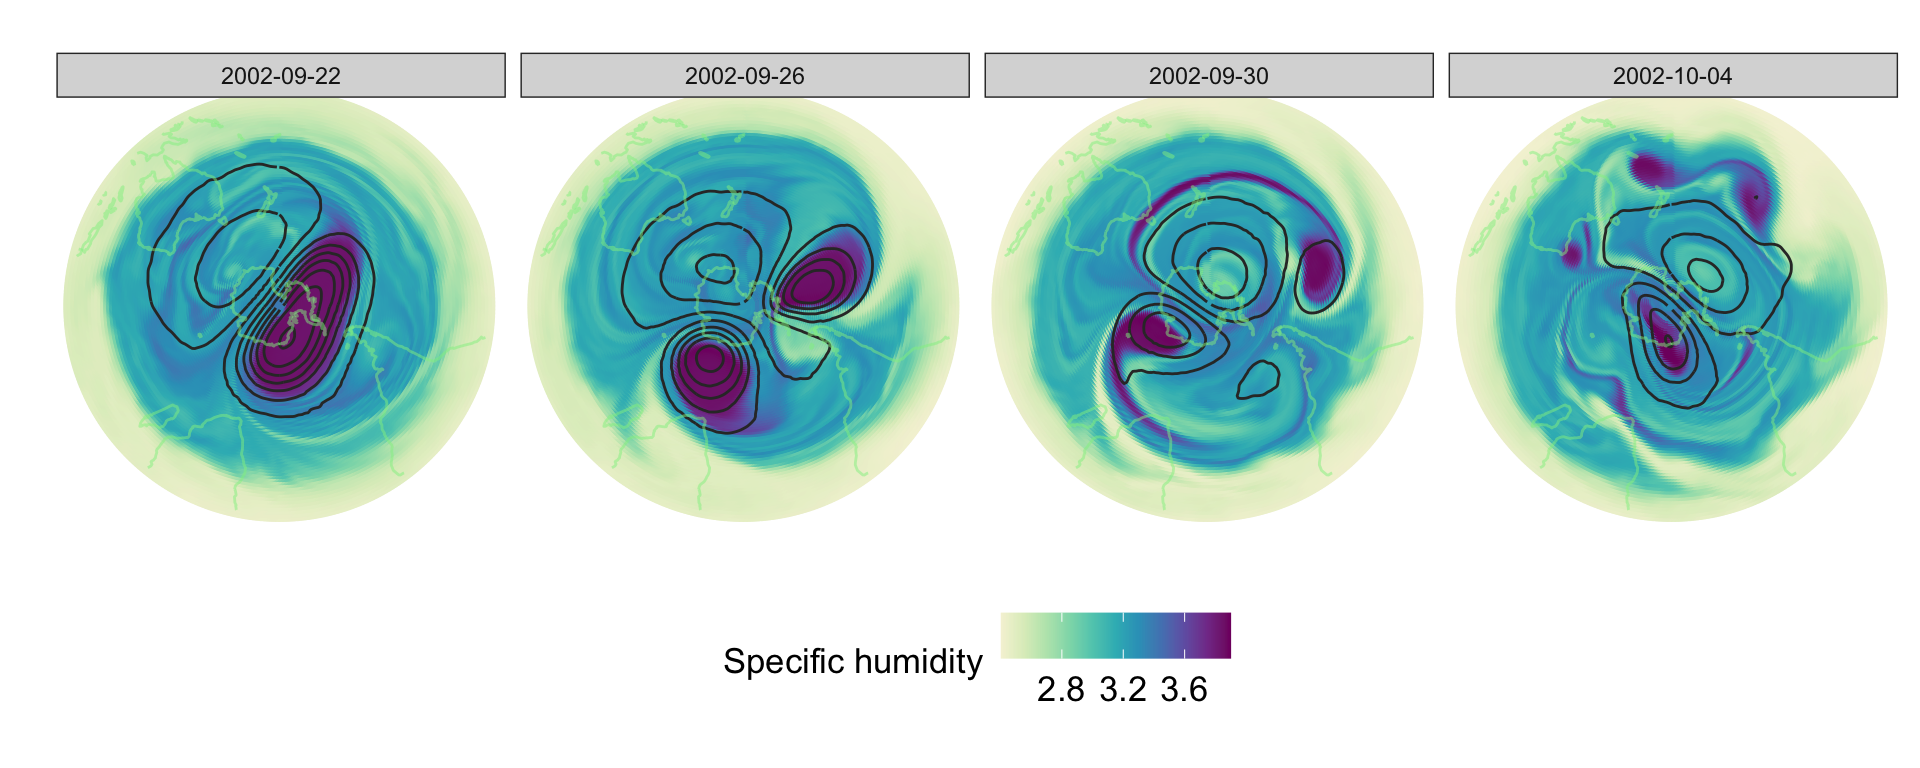
\includegraphics[width=1\linewidth]{/Users/pmen0008/Desktop/paper-cubble/figures/netcdf-1} 

}

\caption[A reproduction of the second row (ERA5 data) of Figure 19 in Hersbach et al (2020) to illustrate the break-up of sourthern polar vortex in late September and early October 2002]{A reproduction of the second row (ERA5 data) of Figure 19 in Hersbach et al (2020) to illustrate the break-up of sourthern polar vortex in late September and early October 2002. The polar vortex, signalled by the high specific humidity, splits into two on 2002-09-26 and further splits into four on 2002-10-04.}\label{fig:netcdf}
\end{figure}
\end{CodeChunk}

\hypertarget{australian-temperature-range}{%
\subsection{Australian temperature range}\label{australian-temperature-range}}

Interactive graphics can be especially useful for spatio-temporal data because they make it possible to look at the data in multiple ways on-the-fly. The last example describes the process of using cubble with the \pkg{crosstalk} package to build an interactive display connecting a map of Australia, with ribbon plots of temperature range observed at the stations in 2020. The purpose is to explore the variation of monthly temperature range over the country.

We will first summarise the daily data in \code{climate_aus} into monthly average and calculate the variance of the temperature difference, which will be used to color the temperature band later.

\begin{verbatim}
clean <- climate_aus |>
  face_temporal() |> 
  mutate(month = lubridate::month(date)) |>
  group_by(month) |>
  summarise(
    tmax = mean(tmax, na.rm = TRUE),
    tmin = mean(tmin, na.rm = TRUE),
    diff = mean(tmax - tmin, na.rm = TRUE)
  ) |> 
  face_spatial() |> 
  rowwise() |>
  mutate(temp_diff_var = var(ts$diff, na.rm =TRUE))
\end{verbatim}

The spatial and temporal cubble are then created into shared \code{crosstalk} objects, plotted as ggplots, and combined together using \code{crosstalk::bscols()}:

\begin{verbatim}
nested <- clean |> SharedData$new(~id, group = "cubble")

long <- clean |> 
  face_temporal() |> 
  SharedData$new(~id, group = "cubble")
  
p1 <- nested |> ggplot() + ...
p2 <- long |> ggplot() + ...
crosstalk::bscols(plotly::ggplotly(p1), plotly::ggplotly(p2), ...)
\end{verbatim}

Figure \ref{fig:interactive-linking} shows three snapshots of the interactivity. Plot (a) shows the initial state of the interactive display: all locations are shown as dots on the map, coloured by the temperature range, and the right plot shows the ribbons representing maximum to minimum for all stations. In plot (b) the station shows a high variance on the initial map, the ``Mount Elizabeth'' station, is selected and this produces the ribbon on the right. In plot (c) the lowest temperature in August is selected on the left map and this corresponds to the ``Thredbo'' station in the mountain area in Victoria and New South Wales. This station is compared to a station in the Tasmania island, the southernmost island of the country, selected on the map.

\begin{CodeChunk}
\begin{figure}

{\centering 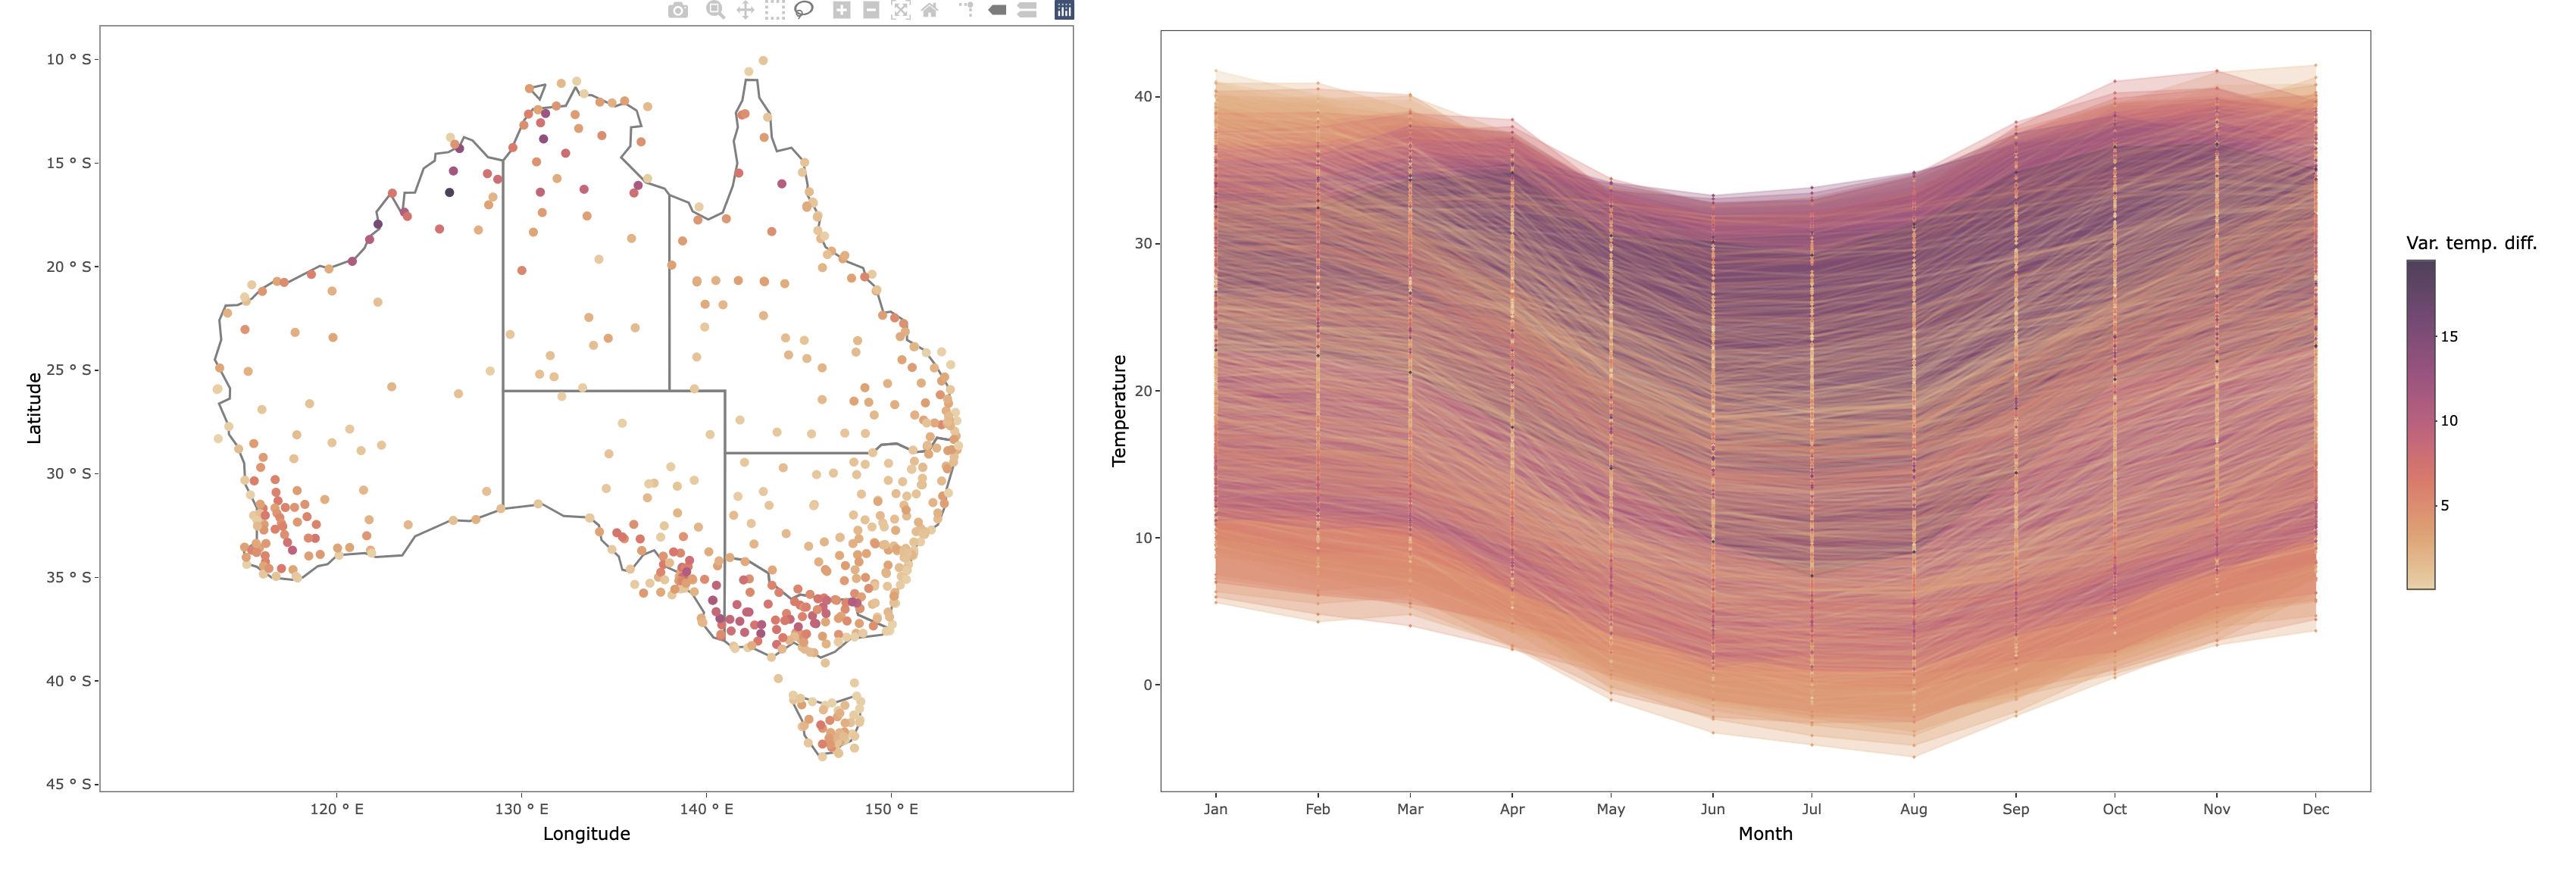
\includegraphics[width=1\linewidth,height=0.23\textheight]{/Users/pmen0008/Desktop/paper-cubble/figures/linking} 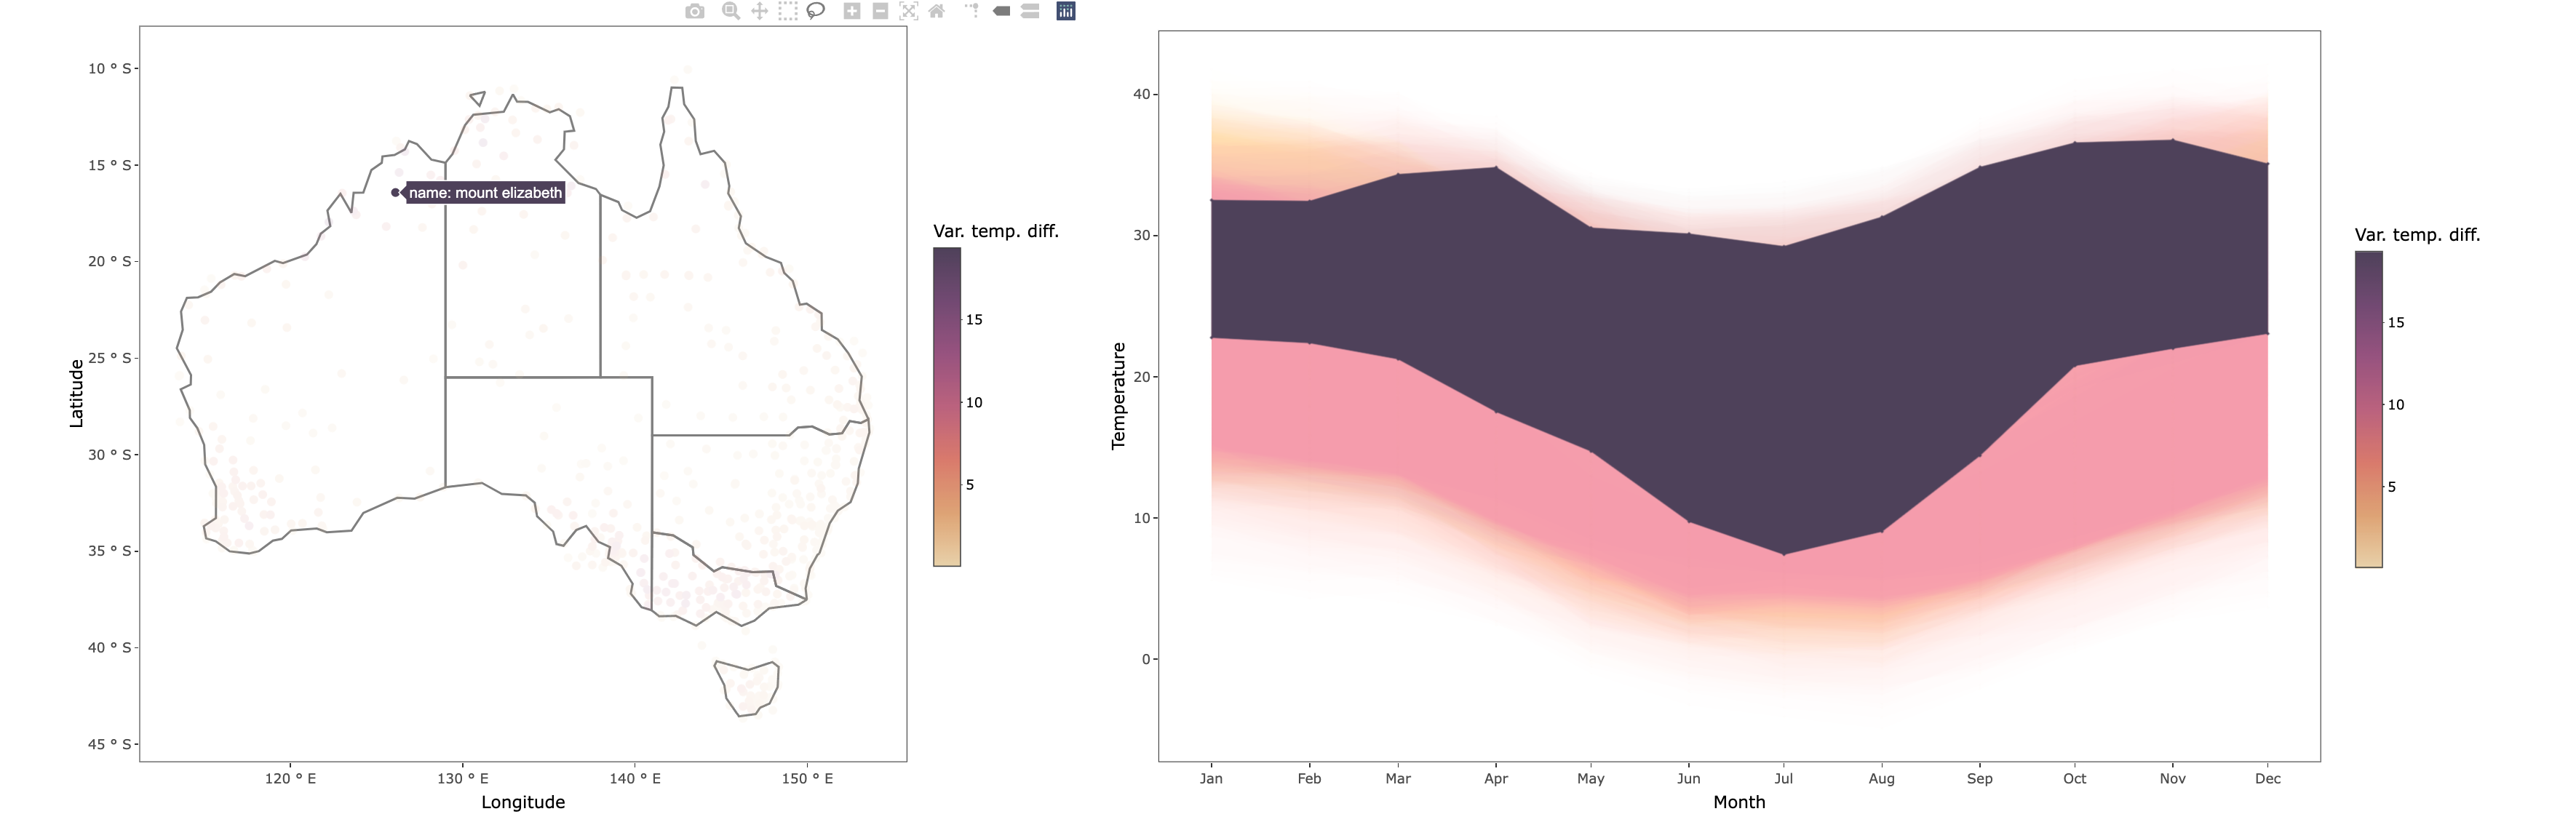
\includegraphics[width=1\linewidth,height=0.23\textheight]{/Users/pmen0008/Desktop/paper-cubble/figures/linking-north} 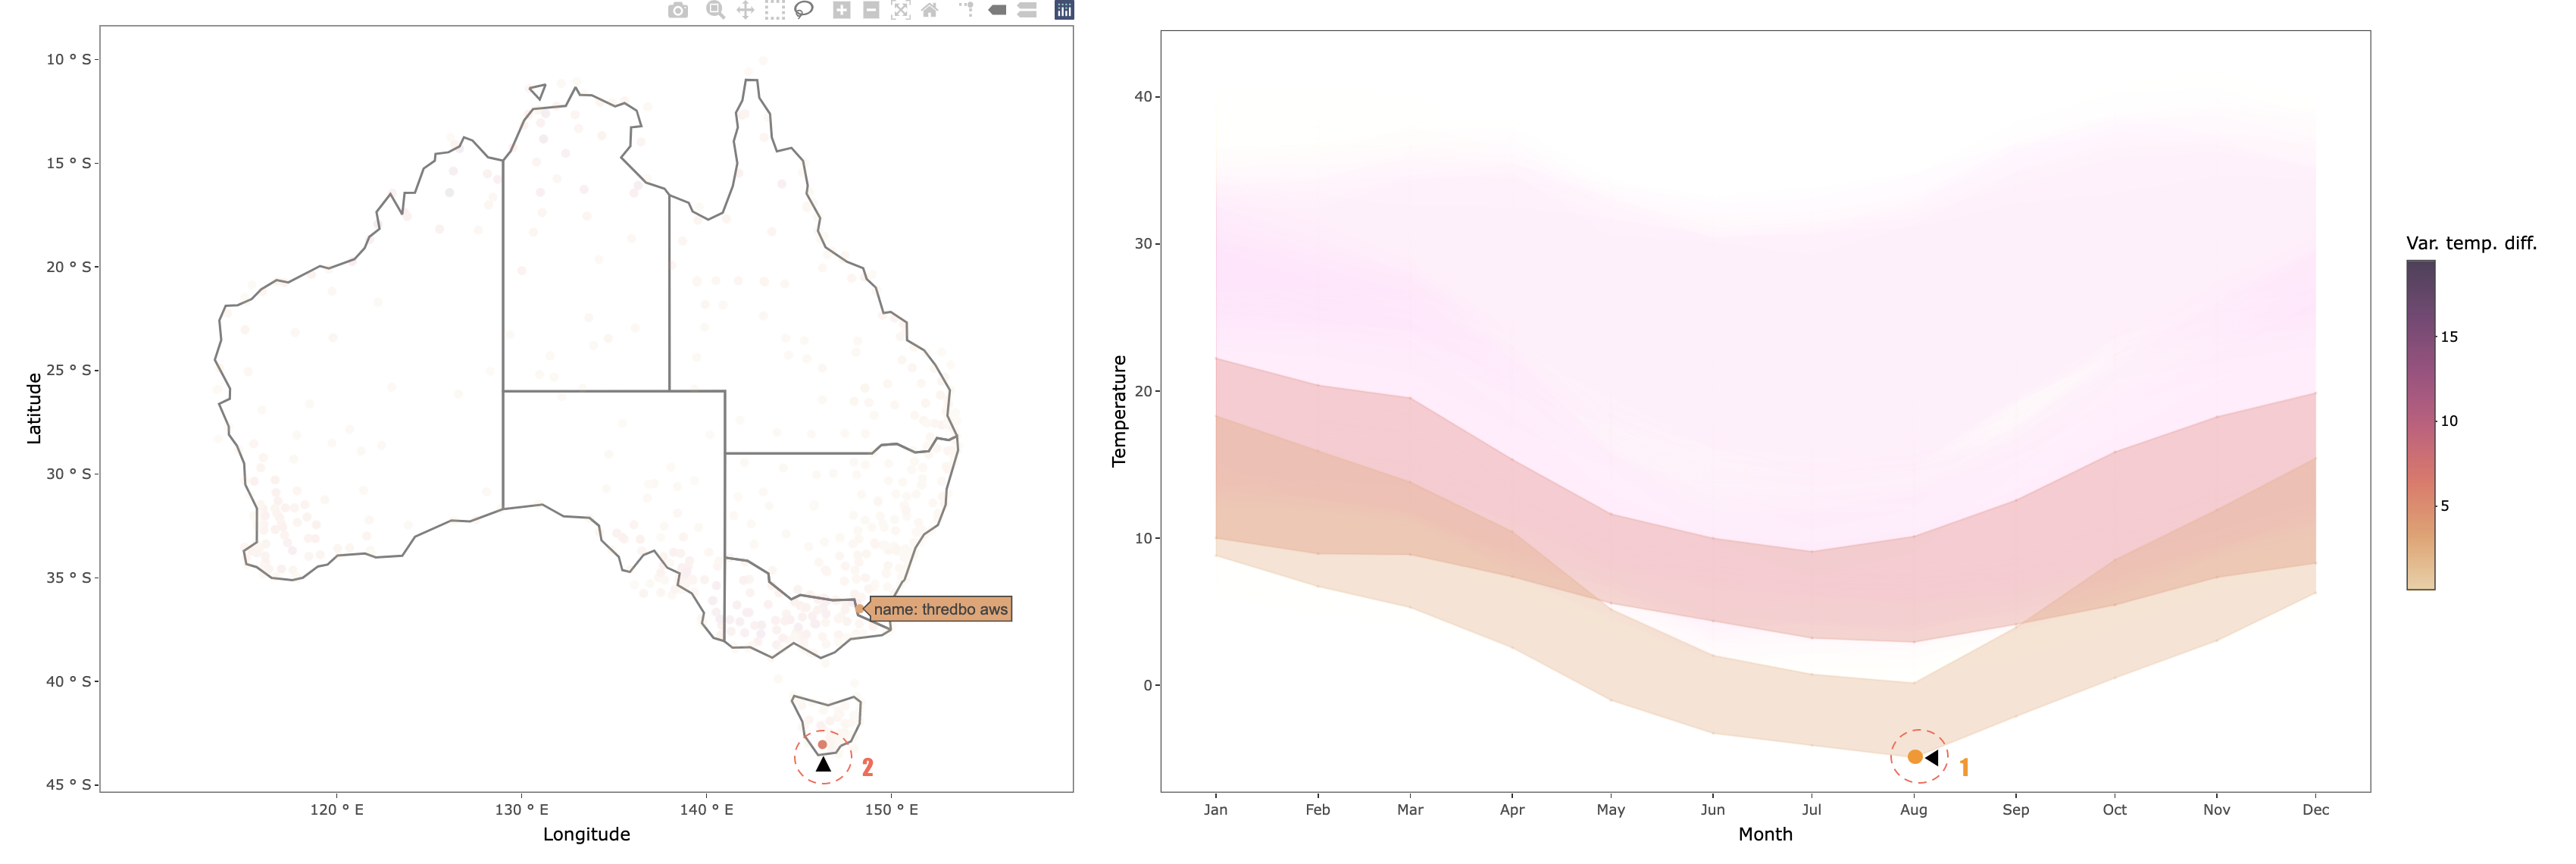
\includegraphics[width=1\linewidth,height=0.23\textheight]{/Users/pmen0008/Desktop/paper-cubble/figures/linking-lower} 

}

\caption[Exploring temperature variation using linking of a map and seasonal display]{Exploring temperature variation using linking of a map and seasonal display. Each row is a screen dump of the process. The top row shows all locations and all temperature profiles. Selecting a particular location on the map (here Mount Elizabeth) produces the plot in the second row. The maximum and minimum temperatures are shown using a ribbon. The bottom row first selects the lowest temperature in August in the seasonal display, which highlights the corresponding station on the map (Thredbo). Another  station, located in the Tasmania Island, is then selected to compare its temperature variation with the Thredbo station.}\label{fig:interactive-linking}
\end{figure}
\end{CodeChunk}

\hypertarget{conclude}{%
\section{Conclusion}\label{conclude}}

This paper presents the \proglang{R} package \pkg{cubble} for organizing, wrangling and visualizing spatio-temporal data. The package introduces a new data structure, \code{cubble}, consisting of two subclass, spatial cubble and a temporal cubble, to organise spatio-temporal data in two different formats within the tidy data framework. The data structure and functions introduced in the package can be used and combined with existing tools for data wrangling, spatial and temporal data analysis, and visualization.

The paper includes plenty examples to illustrate the utility of \pkg{cubble} as a data structure for spatio-temporal analysis. These examples cover different tasks of a typical analysis workflow: handling data with spatial and temporal misalignment, matching data from multiple sources, and creating both static and interactive spatio-temporal visualisation. For future directions, other commonly-used spatial or temporal data structures can be integrated into the \pkg{cubble} package to extend analysts' familiar spatial and temporal toolkit to spatio-temporal.

\hypertarget{acknowledgement}{%
\section{Acknowledgement}\label{acknowledgement}}

This work is funded by a Commonwealth Scientific and Industrial Research Organisation (CSIRO) Data61 Scholarship and started while Nicolas Langrené was affiliated with CSIRO's Data61. The article is created using the package \pkg{knitr} \citep{knitr} and \pkg{rmarkdown} \citep{rmarkdown} in \proglang{R} with the \code{rticles::jss_article} template. The source code for reproducing this paper can be found at: \url{https://github.com/huizezhang-sherry/paper-cubble}.

\bibliography{references.bib}



\end{document}
